\documentclass[]{article}
\usepackage{lmodern}
\usepackage{amssymb,amsmath}
\usepackage{ifxetex,ifluatex}
\usepackage{fixltx2e} % provides \textsubscript
\ifnum 0\ifxetex 1\fi\ifluatex 1\fi=0 % if pdftex
  \usepackage[T1]{fontenc}
  \usepackage[utf8]{inputenc}
\else % if luatex or xelatex
  \ifxetex
    \usepackage{mathspec}
  \else
    \usepackage{fontspec}
  \fi
  \defaultfontfeatures{Ligatures=TeX,Scale=MatchLowercase}
\fi
% use upquote if available, for straight quotes in verbatim environments
\IfFileExists{upquote.sty}{\usepackage{upquote}}{}
% use microtype if available
\IfFileExists{microtype.sty}{%
\usepackage{microtype}
\UseMicrotypeSet[protrusion]{basicmath} % disable protrusion for tt fonts
}{}
\usepackage[margin=1in]{geometry}
\usepackage{hyperref}
\hypersetup{unicode=true,
            pdftitle={Minería de datos: mod01},
            pdfauthor={Autor: Raquel Martín},
            pdfborder={0 0 0},
            breaklinks=true}
\urlstyle{same}  % don't use monospace font for urls
\usepackage{color}
\usepackage{fancyvrb}
\newcommand{\VerbBar}{|}
\newcommand{\VERB}{\Verb[commandchars=\\\{\}]}
\DefineVerbatimEnvironment{Highlighting}{Verbatim}{commandchars=\\\{\}}
% Add ',fontsize=\small' for more characters per line
\usepackage{framed}
\definecolor{shadecolor}{RGB}{48,48,48}
\newenvironment{Shaded}{\begin{snugshade}}{\end{snugshade}}
\newcommand{\AlertTok}[1]{\textcolor[rgb]{1.00,0.81,0.69}{#1}}
\newcommand{\AnnotationTok}[1]{\textcolor[rgb]{0.50,0.62,0.50}{\textbf{#1}}}
\newcommand{\AttributeTok}[1]{\textcolor[rgb]{0.80,0.80,0.80}{#1}}
\newcommand{\BaseNTok}[1]{\textcolor[rgb]{0.86,0.64,0.64}{#1}}
\newcommand{\BuiltInTok}[1]{\textcolor[rgb]{0.80,0.80,0.80}{#1}}
\newcommand{\CharTok}[1]{\textcolor[rgb]{0.86,0.64,0.64}{#1}}
\newcommand{\CommentTok}[1]{\textcolor[rgb]{0.50,0.62,0.50}{#1}}
\newcommand{\CommentVarTok}[1]{\textcolor[rgb]{0.50,0.62,0.50}{\textbf{#1}}}
\newcommand{\ConstantTok}[1]{\textcolor[rgb]{0.86,0.64,0.64}{\textbf{#1}}}
\newcommand{\ControlFlowTok}[1]{\textcolor[rgb]{0.94,0.87,0.69}{#1}}
\newcommand{\DataTypeTok}[1]{\textcolor[rgb]{0.87,0.87,0.75}{#1}}
\newcommand{\DecValTok}[1]{\textcolor[rgb]{0.86,0.86,0.80}{#1}}
\newcommand{\DocumentationTok}[1]{\textcolor[rgb]{0.50,0.62,0.50}{#1}}
\newcommand{\ErrorTok}[1]{\textcolor[rgb]{0.76,0.75,0.62}{#1}}
\newcommand{\ExtensionTok}[1]{\textcolor[rgb]{0.80,0.80,0.80}{#1}}
\newcommand{\FloatTok}[1]{\textcolor[rgb]{0.75,0.75,0.82}{#1}}
\newcommand{\FunctionTok}[1]{\textcolor[rgb]{0.94,0.94,0.56}{#1}}
\newcommand{\ImportTok}[1]{\textcolor[rgb]{0.80,0.80,0.80}{#1}}
\newcommand{\InformationTok}[1]{\textcolor[rgb]{0.50,0.62,0.50}{\textbf{#1}}}
\newcommand{\KeywordTok}[1]{\textcolor[rgb]{0.94,0.87,0.69}{#1}}
\newcommand{\NormalTok}[1]{\textcolor[rgb]{0.80,0.80,0.80}{#1}}
\newcommand{\OperatorTok}[1]{\textcolor[rgb]{0.94,0.94,0.82}{#1}}
\newcommand{\OtherTok}[1]{\textcolor[rgb]{0.94,0.94,0.56}{#1}}
\newcommand{\PreprocessorTok}[1]{\textcolor[rgb]{1.00,0.81,0.69}{\textbf{#1}}}
\newcommand{\RegionMarkerTok}[1]{\textcolor[rgb]{0.80,0.80,0.80}{#1}}
\newcommand{\SpecialCharTok}[1]{\textcolor[rgb]{0.86,0.64,0.64}{#1}}
\newcommand{\SpecialStringTok}[1]{\textcolor[rgb]{0.80,0.58,0.58}{#1}}
\newcommand{\StringTok}[1]{\textcolor[rgb]{0.80,0.58,0.58}{#1}}
\newcommand{\VariableTok}[1]{\textcolor[rgb]{0.80,0.80,0.80}{#1}}
\newcommand{\VerbatimStringTok}[1]{\textcolor[rgb]{0.80,0.58,0.58}{#1}}
\newcommand{\WarningTok}[1]{\textcolor[rgb]{0.50,0.62,0.50}{\textbf{#1}}}
\usepackage{graphicx,grffile}
\makeatletter
\def\maxwidth{\ifdim\Gin@nat@width>\linewidth\linewidth\else\Gin@nat@width\fi}
\def\maxheight{\ifdim\Gin@nat@height>\textheight\textheight\else\Gin@nat@height\fi}
\makeatother
% Scale images if necessary, so that they will not overflow the page
% margins by default, and it is still possible to overwrite the defaults
% using explicit options in \includegraphics[width, height, ...]{}
\setkeys{Gin}{width=\maxwidth,height=\maxheight,keepaspectratio}
\IfFileExists{parskip.sty}{%
\usepackage{parskip}
}{% else
\setlength{\parindent}{0pt}
\setlength{\parskip}{6pt plus 2pt minus 1pt}
}
\setlength{\emergencystretch}{3em}  % prevent overfull lines
\providecommand{\tightlist}{%
  \setlength{\itemsep}{0pt}\setlength{\parskip}{0pt}}
\setcounter{secnumdepth}{0}
% Redefines (sub)paragraphs to behave more like sections
\ifx\paragraph\undefined\else
\let\oldparagraph\paragraph
\renewcommand{\paragraph}[1]{\oldparagraph{#1}\mbox{}}
\fi
\ifx\subparagraph\undefined\else
\let\oldsubparagraph\subparagraph
\renewcommand{\subparagraph}[1]{\oldsubparagraph{#1}\mbox{}}
\fi

%%% Use protect on footnotes to avoid problems with footnotes in titles
\let\rmarkdownfootnote\footnote%
\def\footnote{\protect\rmarkdownfootnote}

%%% Change title format to be more compact
\usepackage{titling}

% Create subtitle command for use in maketitle
\providecommand{\subtitle}[1]{
  \posttitle{
    \begin{center}\large#1\end{center}
    }
}

\setlength{\droptitle}{-2em}

  \title{Minería de datos: mod01}
    \pretitle{\vspace{\droptitle}\centering\huge}
  \posttitle{\par}
    \author{Autor: Raquel Martín}
    \preauthor{\centering\large\emph}
  \postauthor{\par}
      \predate{\centering\large\emph}
  \postdate{\par}
    \date{noviembre 2020}


\begin{document}
\maketitle

{
\setcounter{tocdepth}{2}
\tableofcontents
}
\begin{center}\rule{0.5\linewidth}{0.5pt}\end{center}

\hypertarget{introduccion}{%
\section{Introducción}\label{introduccion}}

\begin{center}\rule{0.5\linewidth}{0.5pt}\end{center}

\hypertarget{descripcion-de-la-practica-a-realizar}{%
\subsection{Descripción de la PRÁCTICA a
realizar}\label{descripcion-de-la-practica-a-realizar}}

La prueba está estructurada en 1 ejercicio teórico/práctico y 1
ejercicio práctico que pide que se desarrolle la fase de preparación en
un juego de datos.\\
Deben responderse todos los ejercicios para poder superar la PRA.

\hypertarget{recursos}{%
\subsection{Recursos}\label{recursos}}

Para realizar esta práctica recomendamos la lectura de los siguientes
documentos:

\begin{itemize}
\tightlist
\item
  RStudio Cheat Sheet: Disponible en el aula Laboratorio de Minería de
  datos.\\
\item
  R Base Cheat Sheet: Disponible en el aula Laboratorio de Minería de
  datos.
\end{itemize}

\begin{center}\rule{0.5\linewidth}{0.5pt}\end{center}

\hypertarget{enunciado}{%
\section{Enunciado}\label{enunciado}}

\begin{center}\rule{0.5\linewidth}{0.5pt}\end{center}

Como ejemplo, trabajaremos con el conjunto de datos ``Titanic'' que
recoge datos sobre el famoso crucero y sobre el que es fácil realizar
tareas de clasificación predictiva sobre la variable ``Survived''.

De momento dejaremos para las siguientes prácticas el estudio de
algoritmos predictivos y nos centraremos por ahora en el estudio de las
variables de una muestra de datos, es decir, haremos un trabajo
descriptivo del mismo.

Las actividades que llevaremos a cabo en esta práctica suelen enmarcarse
en las fases iniciales de un proyecto de minería de datos y consisten en
la selección de caraterísticas o variables y la preparación del los
datos para posteriormente ser consumido por un algoritmo.

Las técnicas que trabajaremos son las siguientes:

\begin{enumerate}
\def\labelenumi{\arabic{enumi}.}
\tightlist
\item
  Normalización\\
\item
  Discretización\\
\item
  Gestión de valores nulos\\
\item
  Estudio de correlaciones\\
\item
  Reducción de la dimensionalidad
\item
  Análisis visual del conjunto de datos
\end{enumerate}

\begin{center}\rule{0.5\linewidth}{0.5pt}\end{center}

\hypertarget{ejemplo-de-estudio-visual-con-el-juego-de-datos-titanic}{%
\section{Ejemplo de estudio visual con el juego de datos
Titanic}\label{ejemplo-de-estudio-visual-con-el-juego-de-datos-titanic}}

\begin{center}\rule{0.5\linewidth}{0.5pt}\end{center}

\hypertarget{procesos-de-limpieza-del-conjunto-de-datos}{%
\subsection{Procesos de limpieza del conjunto de
datos}\label{procesos-de-limpieza-del-conjunto-de-datos}}

Primer contacto con el conjunto de datos, visualizamos su estructura.

\begin{Shaded}
\begin{Highlighting}[]
\CommentTok{\# Cargamos los paquetes R que vamos a usar}
\KeywordTok{library}\NormalTok{(ggplot2)}
\KeywordTok{library}\NormalTok{(dplyr)}

\CommentTok{\# Guardamos el conjunto de datos test y train en un único dataset}
\NormalTok{test \textless{}{-}}\StringTok{ }\KeywordTok{read.csv}\NormalTok{(}\StringTok{"C:/Users/raque/Documents/GitHub/https{-}{-}{-}github.com{-}RaquelMartinDiaz{-}NEOLAND{-}DS2020{-}datalabs/data/titanic{-}test.csv"}\NormalTok{,}\DataTypeTok{stringsAsFactors =} \OtherTok{FALSE}\NormalTok{)}
\NormalTok{train \textless{}{-}}\StringTok{ }\KeywordTok{read.csv}\NormalTok{(}\StringTok{\textquotesingle{}C:/Users/raque/Documents/GitHub/https{-}{-}{-}github.com{-}RaquelMartinDiaz{-}NEOLAND{-}DS2020{-}datalabs/data/titanic{-}train.csv\textquotesingle{}}\NormalTok{, }\DataTypeTok{stringsAsFactors =} \OtherTok{FALSE}\NormalTok{)}

\CommentTok{\# Unimos los dos conjuntos de datos en uno solo}
\NormalTok{totalData \textless{}{-}}\StringTok{ }\KeywordTok{bind\_rows}\NormalTok{(train,test)}
\NormalTok{filas=}\KeywordTok{dim}\NormalTok{(train)[}\DecValTok{1}\NormalTok{]}

\CommentTok{\# Verificamos la estructura del conjunto de datos}
\KeywordTok{str}\NormalTok{(totalData)}
\end{Highlighting}
\end{Shaded}

\begin{verbatim}
## 'data.frame':    1309 obs. of  12 variables:
##  $ PassengerId: int  1 2 3 4 5 6 7 8 9 10 ...
##  $ Survived   : int  0 1 1 1 0 0 0 0 1 1 ...
##  $ Pclass     : int  3 1 3 1 3 3 1 3 3 2 ...
##  $ Name       : chr  "Braund, Mr. Owen Harris" "Cumings, Mrs. John Bradley (Florence Briggs Thayer)" "Heikkinen, Miss. Laina" "Futrelle, Mrs. Jacques Heath (Lily May Peel)" ...
##  $ Sex        : chr  "male" "female" "female" "female" ...
##  $ Age        : num  22 38 26 35 35 NA 54 2 27 14 ...
##  $ SibSp      : int  1 1 0 1 0 0 0 3 0 1 ...
##  $ Parch      : int  0 0 0 0 0 0 0 1 2 0 ...
##  $ Ticket     : chr  "A/5 21171" "PC 17599" "STON/O2. 3101282" "113803" ...
##  $ Fare       : num  7.25 71.28 7.92 53.1 8.05 ...
##  $ Cabin      : chr  "" "C85" "" "C123" ...
##  $ Embarked   : chr  "S" "C" "S" "S" ...
\end{verbatim}

Trabajamos los atributos con valores vacíos.

\begin{Shaded}
\begin{Highlighting}[]
\CommentTok{\# Estadísticas de valores vacíos}
\KeywordTok{colSums}\NormalTok{(}\KeywordTok{is.na}\NormalTok{(totalData))}
\end{Highlighting}
\end{Shaded}

\begin{verbatim}
## PassengerId    Survived      Pclass        Name         Sex         Age 
##           0         418           0           0           0         263 
##       SibSp       Parch      Ticket        Fare       Cabin    Embarked 
##           0           0           0           1           0           0
\end{verbatim}

\begin{Shaded}
\begin{Highlighting}[]
\KeywordTok{colSums}\NormalTok{(totalData}\OperatorTok{==}\StringTok{""}\NormalTok{)}
\end{Highlighting}
\end{Shaded}

\begin{verbatim}
## PassengerId    Survived      Pclass        Name         Sex         Age 
##           0          NA           0           0           0          NA 
##       SibSp       Parch      Ticket        Fare       Cabin    Embarked 
##           0           0           0          NA        1014           2
\end{verbatim}

\begin{Shaded}
\begin{Highlighting}[]
\CommentTok{\# Tomamos valor "C" para los valores vacíos de la variable "Embarked"}
\NormalTok{totalData}\OperatorTok{$}\NormalTok{Embarked[totalData}\OperatorTok{$}\NormalTok{Embarked}\OperatorTok{==}\StringTok{""}\NormalTok{]=}\StringTok{"C"}

\CommentTok{\# Tomamos la media para valores vacíos de la variable "Age"}
\NormalTok{totalData}\OperatorTok{$}\NormalTok{Age[}\KeywordTok{is.na}\NormalTok{(totalData}\OperatorTok{$}\NormalTok{Age)] \textless{}{-}}\StringTok{ }\KeywordTok{mean}\NormalTok{(totalData}\OperatorTok{$}\NormalTok{Age,}\DataTypeTok{na.rm=}\NormalTok{T)}
\end{Highlighting}
\end{Shaded}

Discretizamos cuando tiene sentido y en función de cada variable.

\begin{Shaded}
\begin{Highlighting}[]
\CommentTok{\# ¿Con qué variables tendría sentido un proceso de discretización?}
\KeywordTok{apply}\NormalTok{(totalData,}\DecValTok{2}\NormalTok{, }\ControlFlowTok{function}\NormalTok{(x) }\KeywordTok{length}\NormalTok{(}\KeywordTok{unique}\NormalTok{(x)))}
\end{Highlighting}
\end{Shaded}

\begin{verbatim}
## PassengerId    Survived      Pclass        Name         Sex         Age 
##        1309           3           3        1307           2          99 
##       SibSp       Parch      Ticket        Fare       Cabin    Embarked 
##           7           8         929         282         187           3
\end{verbatim}

\begin{Shaded}
\begin{Highlighting}[]
\CommentTok{\# Discretizamos las variables con pocas clases}
\NormalTok{cols\textless{}{-}}\KeywordTok{c}\NormalTok{(}\StringTok{"Survived"}\NormalTok{,}\StringTok{"Pclass"}\NormalTok{,}\StringTok{"Sex"}\NormalTok{,}\StringTok{"Embarked"}\NormalTok{)}
\ControlFlowTok{for}\NormalTok{ (i }\ControlFlowTok{in}\NormalTok{ cols)\{}
\NormalTok{  totalData[,i] \textless{}{-}}\StringTok{ }\KeywordTok{as.factor}\NormalTok{(totalData[,i])}
\NormalTok{\}}

\CommentTok{\# Después de los cambios, analizamos la nueva estructura del conjunto de datos}
\KeywordTok{str}\NormalTok{(totalData)}
\end{Highlighting}
\end{Shaded}

\begin{verbatim}
## 'data.frame':    1309 obs. of  12 variables:
##  $ PassengerId: int  1 2 3 4 5 6 7 8 9 10 ...
##  $ Survived   : Factor w/ 2 levels "0","1": 1 2 2 2 1 1 1 1 2 2 ...
##  $ Pclass     : Factor w/ 3 levels "1","2","3": 3 1 3 1 3 3 1 3 3 2 ...
##  $ Name       : chr  "Braund, Mr. Owen Harris" "Cumings, Mrs. John Bradley (Florence Briggs Thayer)" "Heikkinen, Miss. Laina" "Futrelle, Mrs. Jacques Heath (Lily May Peel)" ...
##  $ Sex        : Factor w/ 2 levels "female","male": 2 1 1 1 2 2 2 2 1 1 ...
##  $ Age        : num  22 38 26 35 35 ...
##  $ SibSp      : int  1 1 0 1 0 0 0 3 0 1 ...
##  $ Parch      : int  0 0 0 0 0 0 0 1 2 0 ...
##  $ Ticket     : chr  "A/5 21171" "PC 17599" "STON/O2. 3101282" "113803" ...
##  $ Fare       : num  7.25 71.28 7.92 53.1 8.05 ...
##  $ Cabin      : chr  "" "C85" "" "C123" ...
##  $ Embarked   : Factor w/ 3 levels "C","Q","S": 3 1 3 3 3 2 3 3 3 1 ...
\end{verbatim}

\hypertarget{procesos-de-analisis-del-conjunto-de-datos}{%
\subsection{Procesos de análisis del conjunto de
datos}\label{procesos-de-analisis-del-conjunto-de-datos}}

Nos proponemos analizar las relaciones entre las diferentes variables
del conjunto de datos.

\begin{Shaded}
\begin{Highlighting}[]
\CommentTok{\# Visualizamos la relación entre las variables "sex" y "survival":}
\KeywordTok{ggplot}\NormalTok{(}\DataTypeTok{data=}\NormalTok{totalData[}\DecValTok{1}\OperatorTok{:}\NormalTok{filas,],}\KeywordTok{aes}\NormalTok{(}\DataTypeTok{x=}\NormalTok{Sex,}\DataTypeTok{fill=}\NormalTok{Survived))}\OperatorTok{+}\KeywordTok{geom\_bar}\NormalTok{()}
\end{Highlighting}
\end{Shaded}

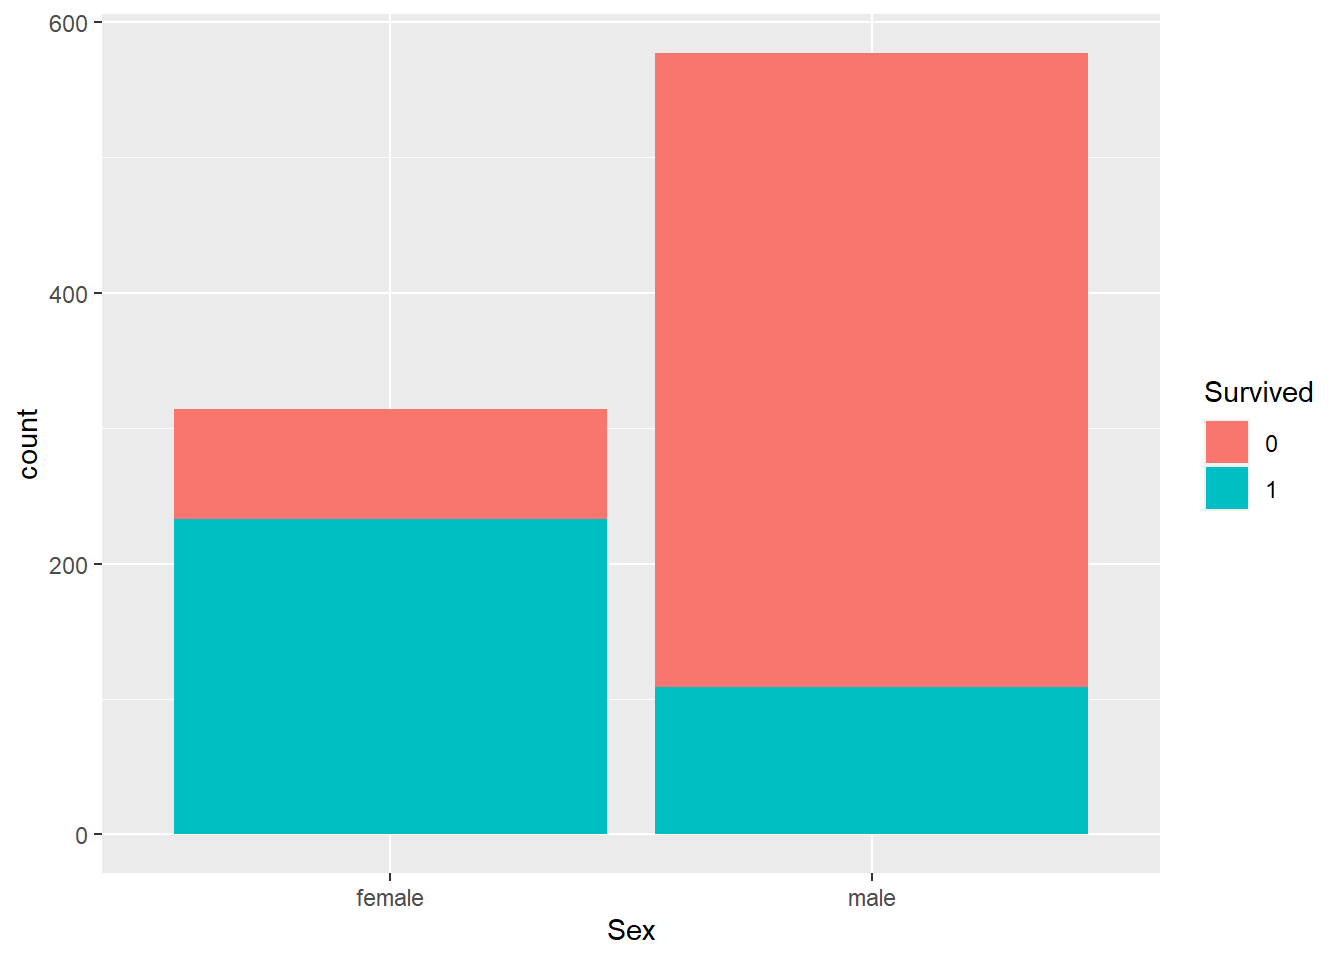
\includegraphics{pra01_Raquel_files/figure-latex/unnamed-chunk-4-1.pdf}

\begin{Shaded}
\begin{Highlighting}[]
\CommentTok{\# Otro punto de vista. Survival como función de Embarked:}
\KeywordTok{ggplot}\NormalTok{(}\DataTypeTok{data =}\NormalTok{ totalData[}\DecValTok{1}\OperatorTok{:}\NormalTok{filas,],}\KeywordTok{aes}\NormalTok{(}\DataTypeTok{x=}\NormalTok{Embarked,}\DataTypeTok{fill=}\NormalTok{Survived))}\OperatorTok{+}\KeywordTok{geom\_bar}\NormalTok{(}\DataTypeTok{position=}\StringTok{"fill"}\NormalTok{)}\OperatorTok{+}\KeywordTok{ylab}\NormalTok{(}\StringTok{"Frecuencia"}\NormalTok{)}
\end{Highlighting}
\end{Shaded}

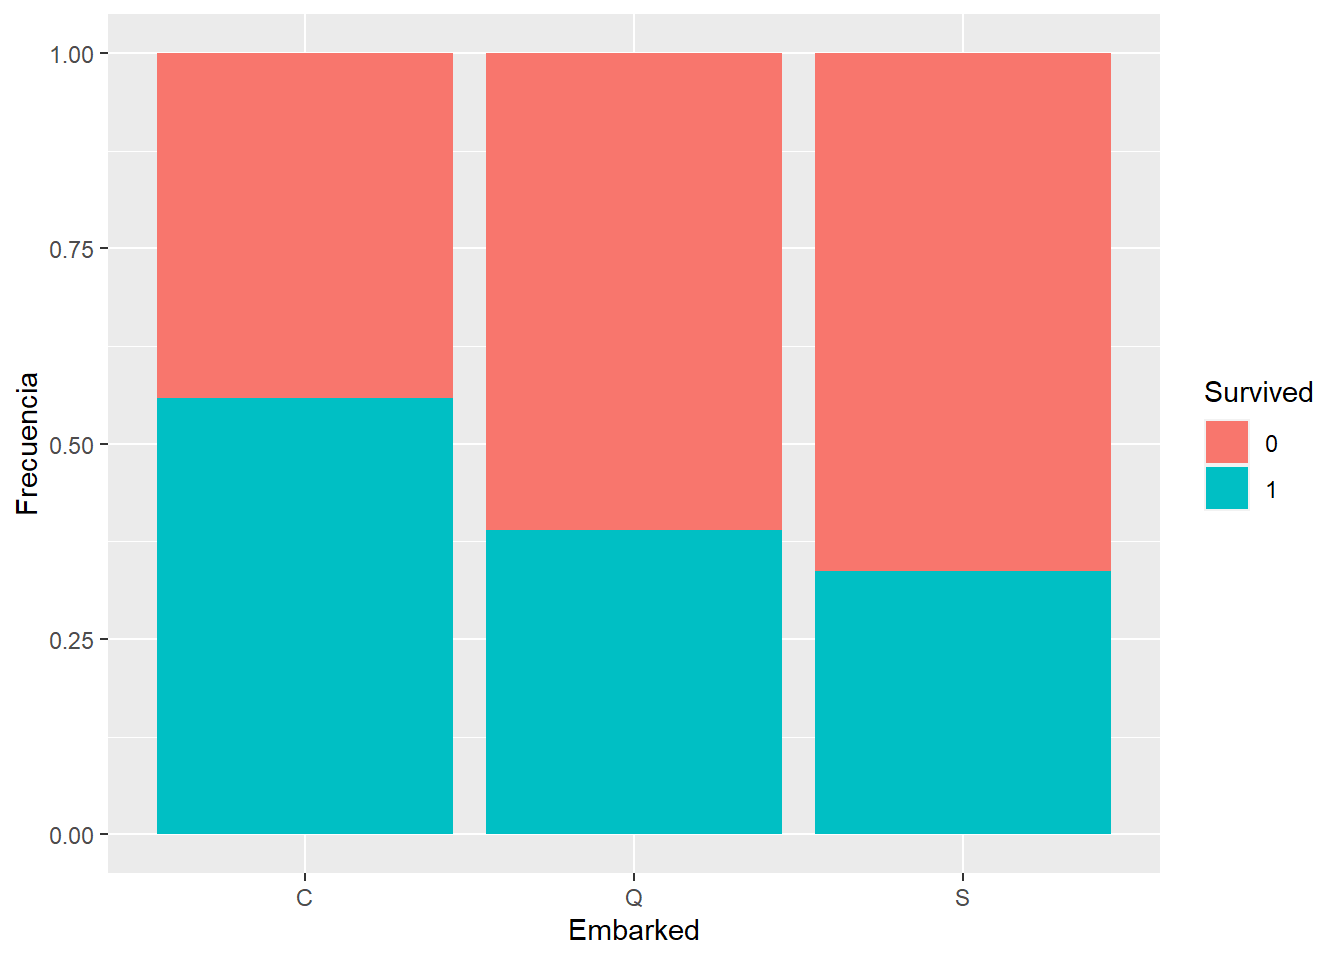
\includegraphics{pra01_Raquel_files/figure-latex/unnamed-chunk-4-2.pdf}

Obtenemos una matriz de porcentages de frecuencia.\\
Vemos, por ejemplo que la probabilidad de sobrevivir si se embarcó en
``C'' es de un 55,88\%

\begin{Shaded}
\begin{Highlighting}[]
\NormalTok{t\textless{}{-}}\KeywordTok{table}\NormalTok{(totalData[}\DecValTok{1}\OperatorTok{:}\NormalTok{filas,]}\OperatorTok{$}\NormalTok{Embarked,totalData[}\DecValTok{1}\OperatorTok{:}\NormalTok{filas,]}\OperatorTok{$}\NormalTok{Survived)}
\ControlFlowTok{for}\NormalTok{ (i }\ControlFlowTok{in} \DecValTok{1}\OperatorTok{:}\KeywordTok{dim}\NormalTok{(t)[}\DecValTok{1}\NormalTok{])\{}
\NormalTok{    t[i,]\textless{}{-}t[i,]}\OperatorTok{/}\KeywordTok{sum}\NormalTok{(t[i,])}\OperatorTok{*}\DecValTok{100}
\NormalTok{\}}
\NormalTok{t}
\end{Highlighting}
\end{Shaded}

\begin{verbatim}
##    
##            0        1
##   C 44.11765 55.88235
##   Q 61.03896 38.96104
##   S 66.30435 33.69565
\end{verbatim}

Veamos ahora como en un mismo gráfico de frecuencias podemos trabajar
con 3 variables: Embarked, Survived y Pclass.

\begin{Shaded}
\begin{Highlighting}[]
\CommentTok{\# Ahora, podemos dividir el gráfico de Embarked por Pclass:}
\KeywordTok{ggplot}\NormalTok{(}\DataTypeTok{data =}\NormalTok{ totalData[}\DecValTok{1}\OperatorTok{:}\NormalTok{filas,],}\KeywordTok{aes}\NormalTok{(}\DataTypeTok{x=}\NormalTok{Embarked,}\DataTypeTok{fill=}\NormalTok{Survived))}\OperatorTok{+}\KeywordTok{geom\_bar}\NormalTok{(}\DataTypeTok{position=}\StringTok{"fill"}\NormalTok{)}\OperatorTok{+}\KeywordTok{facet\_wrap}\NormalTok{(}\OperatorTok{\textasciitilde{}}\NormalTok{Pclass)}
\end{Highlighting}
\end{Shaded}

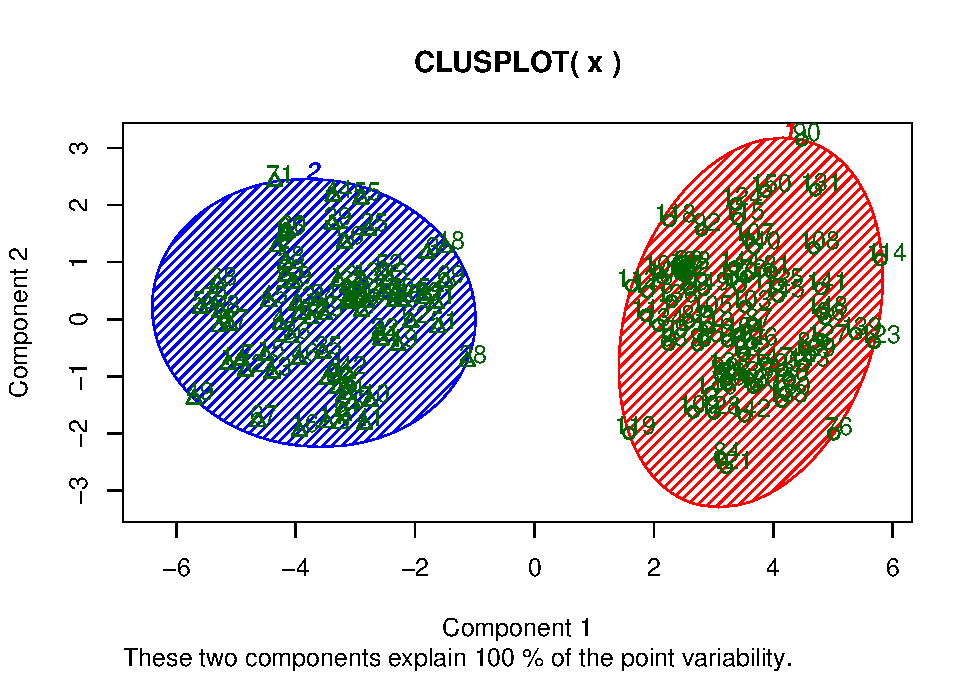
\includegraphics{pra01_Raquel_files/figure-latex/unnamed-chunk-6-1.pdf}

Comparemos ahora dos gráficos de frecuencias: Survived-SibSp y
Survived-Parch

\begin{Shaded}
\begin{Highlighting}[]
\CommentTok{\# Survivial como función de SibSp y Parch}
\KeywordTok{ggplot}\NormalTok{(}\DataTypeTok{data =}\NormalTok{ totalData[}\DecValTok{1}\OperatorTok{:}\NormalTok{filas,],}\KeywordTok{aes}\NormalTok{(}\DataTypeTok{x=}\NormalTok{SibSp,}\DataTypeTok{fill=}\NormalTok{Survived))}\OperatorTok{+}\KeywordTok{geom\_bar}\NormalTok{()}
\end{Highlighting}
\end{Shaded}

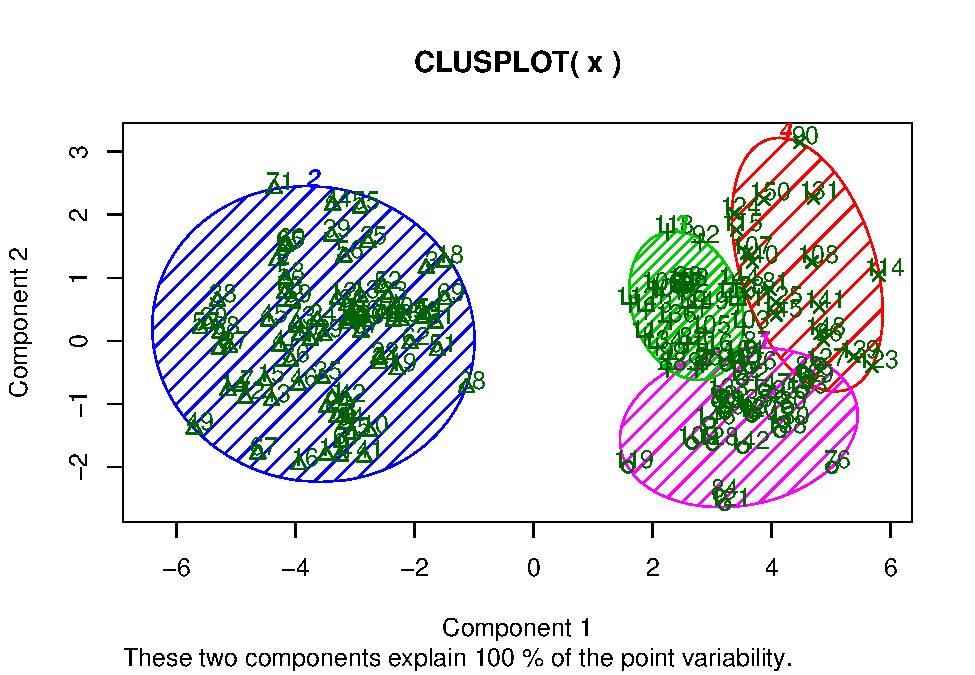
\includegraphics{pra01_Raquel_files/figure-latex/unnamed-chunk-7-1.pdf}

\begin{Shaded}
\begin{Highlighting}[]
\KeywordTok{ggplot}\NormalTok{(}\DataTypeTok{data =}\NormalTok{ totalData[}\DecValTok{1}\OperatorTok{:}\NormalTok{filas,],}\KeywordTok{aes}\NormalTok{(}\DataTypeTok{x=}\NormalTok{Parch,}\DataTypeTok{fill=}\NormalTok{Survived))}\OperatorTok{+}\KeywordTok{geom\_bar}\NormalTok{()}
\end{Highlighting}
\end{Shaded}

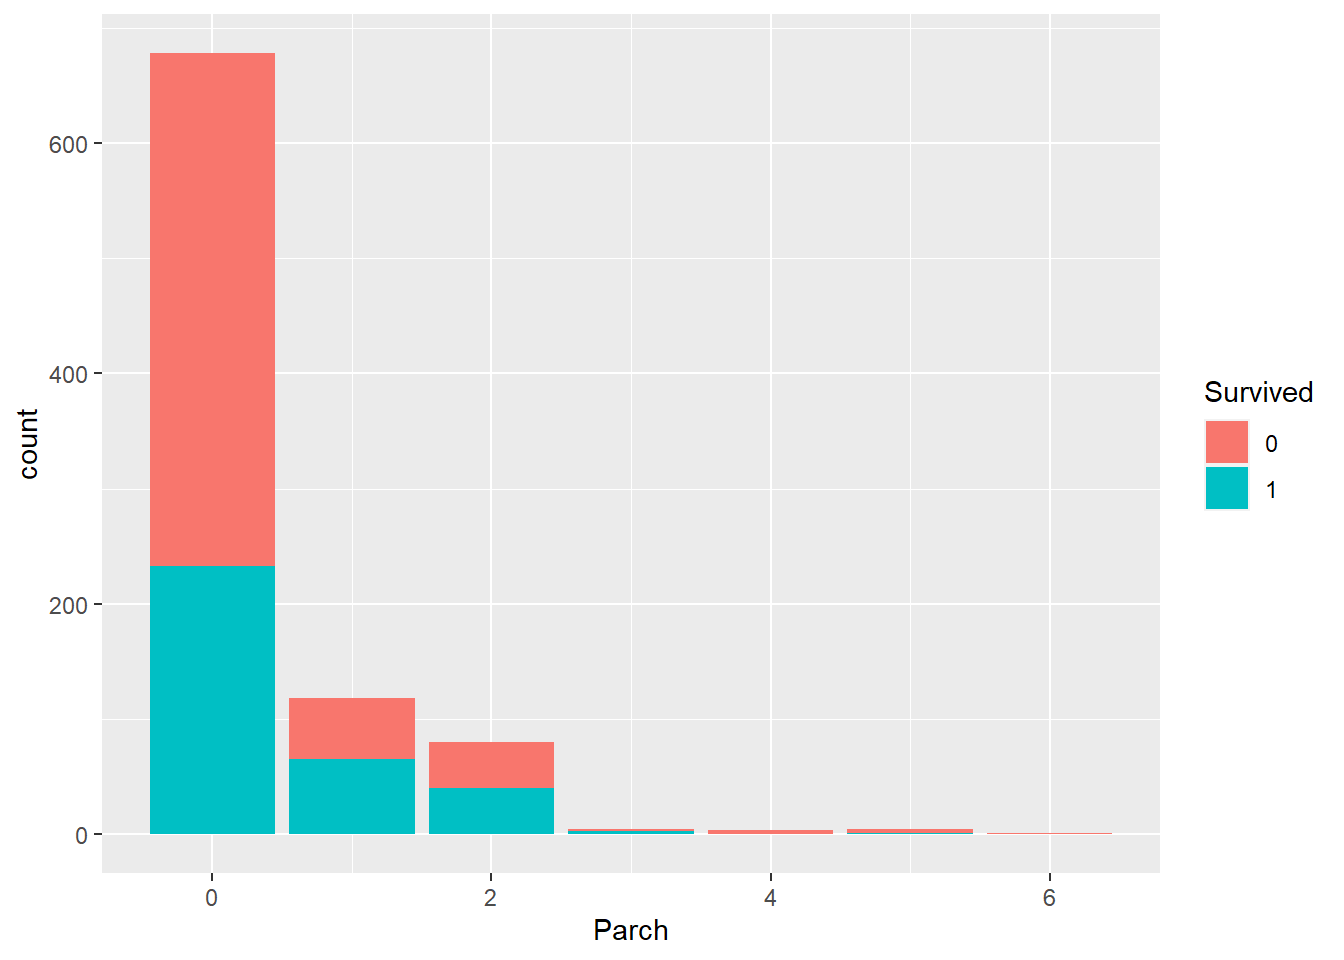
\includegraphics{pra01_Raquel_files/figure-latex/unnamed-chunk-7-2.pdf}

\begin{Shaded}
\begin{Highlighting}[]
\CommentTok{\# Vemos como las forma de estos dos gráficos es similar. Este hecho nos puede indicar presencia de correlaciones altas.}
\end{Highlighting}
\end{Shaded}

Veamos un ejemplo de construcción de una variable nueva: Tamaño de
familia

\begin{Shaded}
\begin{Highlighting}[]
\CommentTok{\# Construimos un atributo nuevo: family size.}
\NormalTok{totalData}\OperatorTok{$}\NormalTok{FamilySize \textless{}{-}}\StringTok{ }\NormalTok{totalData}\OperatorTok{$}\NormalTok{SibSp }\OperatorTok{+}\StringTok{ }\NormalTok{totalData}\OperatorTok{$}\NormalTok{Parch }\OperatorTok{+}\DecValTok{1}\NormalTok{;}
\NormalTok{totalData1\textless{}{-}totalData[}\DecValTok{1}\OperatorTok{:}\NormalTok{filas,]}
\KeywordTok{ggplot}\NormalTok{(}\DataTypeTok{data =}\NormalTok{ totalData1[}\OperatorTok{!}\KeywordTok{is.na}\NormalTok{(totalData[}\DecValTok{1}\OperatorTok{:}\NormalTok{filas,]}\OperatorTok{$}\NormalTok{FamilySize),],}\KeywordTok{aes}\NormalTok{(}\DataTypeTok{x=}\NormalTok{FamilySize,}\DataTypeTok{fill=}\NormalTok{Survived))}\OperatorTok{+}\KeywordTok{geom\_histogram}\NormalTok{(}\DataTypeTok{binwidth =}\DecValTok{1}\NormalTok{,}\DataTypeTok{position=}\StringTok{"fill"}\NormalTok{)}\OperatorTok{+}\KeywordTok{ylab}\NormalTok{(}\StringTok{"Frecuencia"}\NormalTok{)}
\end{Highlighting}
\end{Shaded}

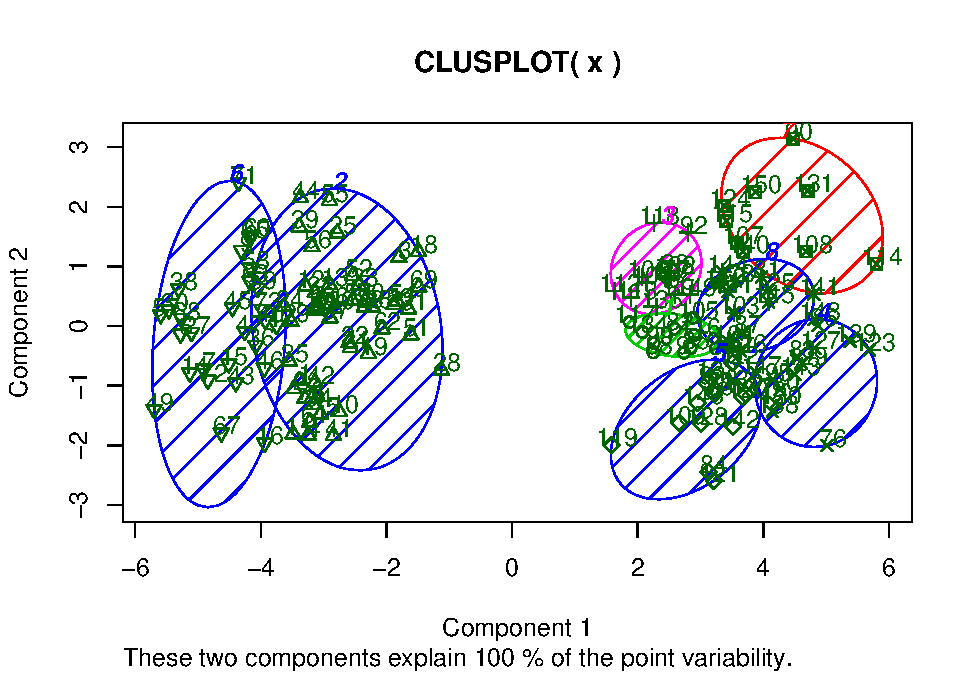
\includegraphics{pra01_Raquel_files/figure-latex/unnamed-chunk-8-1.pdf}

\begin{Shaded}
\begin{Highlighting}[]
\CommentTok{\# Observamos como familias de entre 2 y 6 miembros tienen más del 50\% de posibilidades de supervivencia.  }
\end{Highlighting}
\end{Shaded}

Veamos ahora dos gráficos que nos compara los atributos Age y
Survived.\\
Observamos como el parámetro position=``fill'' nos da la proporción
acumulada de un atributo dentro de otro

\begin{Shaded}
\begin{Highlighting}[]
\CommentTok{\# Survival como función de age:}
\KeywordTok{ggplot}\NormalTok{(}\DataTypeTok{data =}\NormalTok{ totalData1[}\OperatorTok{!}\NormalTok{(}\KeywordTok{is.na}\NormalTok{(totalData[}\DecValTok{1}\OperatorTok{:}\NormalTok{filas,]}\OperatorTok{$}\NormalTok{Age)),],}\KeywordTok{aes}\NormalTok{(}\DataTypeTok{x=}\NormalTok{Age,}\DataTypeTok{fill=}\NormalTok{Survived))}\OperatorTok{+}\KeywordTok{geom\_histogram}\NormalTok{(}\DataTypeTok{binwidth =}\DecValTok{3}\NormalTok{)}
\end{Highlighting}
\end{Shaded}

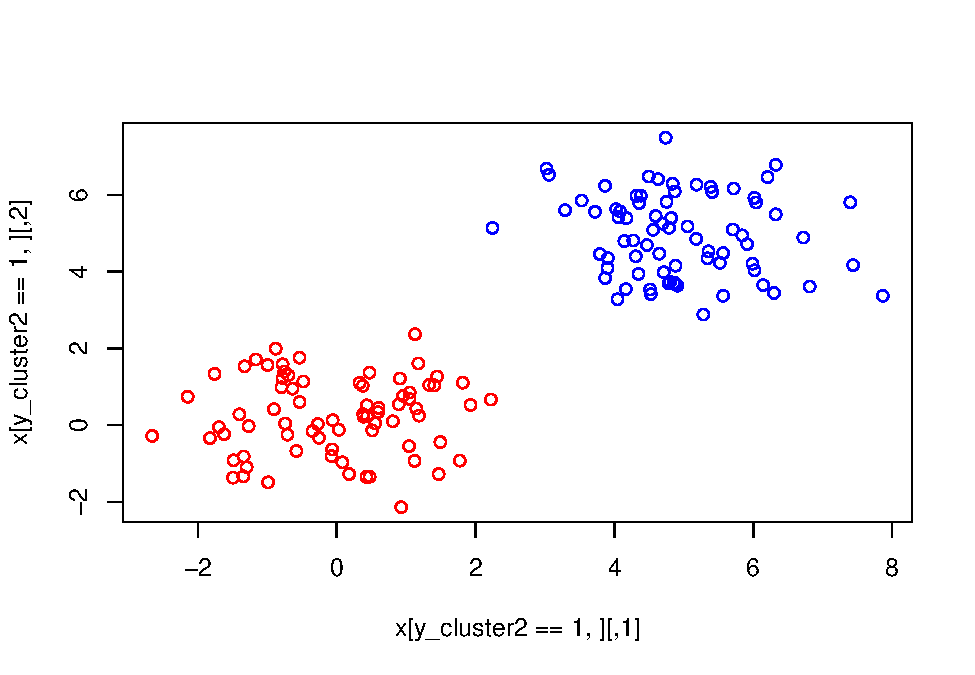
\includegraphics{pra01_Raquel_files/figure-latex/unnamed-chunk-9-1.pdf}

\begin{Shaded}
\begin{Highlighting}[]
\KeywordTok{ggplot}\NormalTok{(}\DataTypeTok{data =}\NormalTok{ totalData1[}\OperatorTok{!}\KeywordTok{is.na}\NormalTok{(totalData[}\DecValTok{1}\OperatorTok{:}\NormalTok{filas,]}\OperatorTok{$}\NormalTok{Age),],}\KeywordTok{aes}\NormalTok{(}\DataTypeTok{x=}\NormalTok{Age,}\DataTypeTok{fill=}\NormalTok{Survived))}\OperatorTok{+}\KeywordTok{geom\_histogram}\NormalTok{(}\DataTypeTok{binwidth =} \DecValTok{3}\NormalTok{,}\DataTypeTok{position=}\StringTok{"fill"}\NormalTok{)}\OperatorTok{+}\KeywordTok{ylab}\NormalTok{(}\StringTok{"Frecuencia"}\NormalTok{)}
\end{Highlighting}
\end{Shaded}

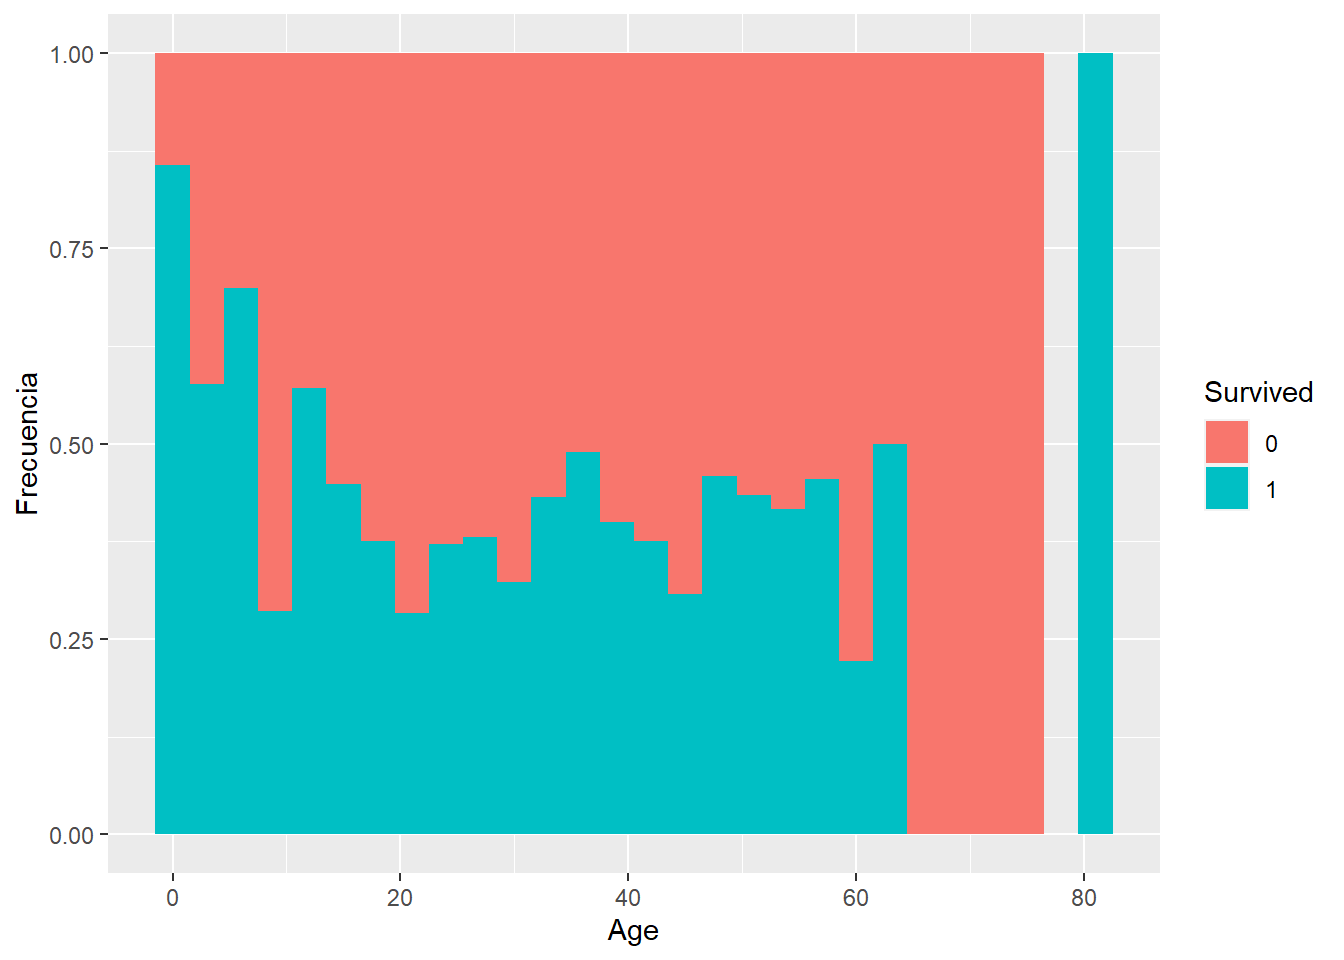
\includegraphics{pra01_Raquel_files/figure-latex/unnamed-chunk-9-2.pdf}

\begin{center}\rule{0.5\linewidth}{0.5pt}\end{center}

\hypertarget{ejercicios}{%
\section{Ejercicios}\label{ejercicios}}

\begin{center}\rule{0.5\linewidth}{0.5pt}\end{center}

\hypertarget{ejercicio-1}{%
\subsection{Ejercicio 1:}\label{ejercicio-1}}

Estudia los tres casos siguientes y contesta, de forma razonada la
pregunta que se realiza:

\begin{itemize}
\item
  Disponemos de un conjunto de variables referentes a vehículos, tales
  como la marca, modelo, año de matriculación, etc. También se dispone
  del precio al que se vendieron. Al poner a la venta a un nuevo
  vehículo, se dispone de las variables que lo describen, pero se
  desconoce el precio. ¿Qué tipo de algoritmo se debería aplicar para
  predecir de forma automática el precio?
\item
  En un almacén de naranjas se tiene una máquina, que de forma
  automática obtiene un conjunto de variables de cada naranja, como su
  tamaño, acidez, grado maduración, etc. Si se desea estudiar las
  naranjas por tipos, según las variables obtenidas, ¿qué tipo de
  algoritmo es el más adecuado?
\item
  Un servicio de música por internet dispone de los historiales de
  audición de sus clientes: Qué canciones y qué grupos eligen los
  clientes a lo largo del tiempo de sus escuchas. La empresa desea crear
  un sistema que proponga la siguiente canción y grupo en función de la
  canción que se ha escuchado antes. ¿Qué tipo de algoritmo es el más
  adecuado?
\end{itemize}

\hypertarget{respuesta-1}{%
\subsubsection{Respuesta 1:}\label{respuesta-1}}

\begin{quote}
Escribe aquí la respuesta a la pregunta
\end{quote}

No termino de entender si quieres que investiguemos acerca de algoritmos
de predicción o lo que haríamos. 1.1.- En el primer caso referente a los
vehículos, estudiaría primero la variable del precio de compra inicial
para ver si tengo NA. Si no tuviera, estudiaría la relación con el resto
de variables, para ver la relación con el modelo, el año de
matriculación, la marca, etc. Luego buscaría información acerca de la
pérdida de valor de un coche con el paso del tiempo, el kilometraje,
etc. Y a partir de ahí crearía una nueva variable con el precio de venta
relacionada con los datos anteriormente objetinos. Si la variable precio
de compra inicial tuviera NA primero comprobaría si tengo datos
duplicados con el resto de variables que sí tengan el precio de compra.
Si no fuera el caso, revisaría por modelos coches similares para estimar
el precio de compra.

\hypertarget{ejercicio-2}{%
\subsection{Ejercicio 2:}\label{ejercicio-2}}

A partir del conjunto de datos disponible en el siguiente enlace
\url{http://archive.ics.uci.edu/ml/datasets/Adult} , realiza un estudio
tomando como propuesta inicial al que se ha realizado con el conjunto de
datos ``Titanic''. Amplia la propuesta generando nuevos indicadores o
solucionando otros problemas expuestos en el módulo 2. Explica el
proceso que has seguido, qué conocimiento obtienes de los datos, qué
objetivo te has fijado y detalla los pasos, técnicas usadas y los
problemas resueltos.

Nota: Si lo deseas puedes utilizar otro conjunto de datos propio o de
algun repositorio open data siempre que sea similar en diversidad de
tipos de variables al propuesto.

\hypertarget{respuesta-2}{%
\subsubsection{Respuesta 2:}\label{respuesta-2}}

\begin{Shaded}
\begin{Highlighting}[]
\CommentTok{\# Cargamos el juego de datos}
\NormalTok{datosAdult \textless{}{-}}\StringTok{ }\KeywordTok{read.csv}\NormalTok{(}\StringTok{\textquotesingle{}http://archive.ics.uci.edu/ml/machine{-}learning{-}databases/adult/adult.data\textquotesingle{}}\NormalTok{,}\DataTypeTok{stringsAsFactors =} \OtherTok{FALSE}\NormalTok{, }\DataTypeTok{header =} \OtherTok{FALSE}\NormalTok{)}

\CommentTok{\# Nombres de los atributos}
\KeywordTok{names}\NormalTok{(datosAdult) \textless{}{-}}\StringTok{ }\KeywordTok{c}\NormalTok{(}\StringTok{"age"}\NormalTok{,}\StringTok{"workclass"}\NormalTok{,}\StringTok{"fnlwgt"}\NormalTok{,}\StringTok{"education"}\NormalTok{,}\StringTok{"education{-}num"}\NormalTok{,}\StringTok{"marital{-}status"}\NormalTok{,}\StringTok{"occupation"}\NormalTok{,}\StringTok{"relationship"}\NormalTok{,}\StringTok{"race"}\NormalTok{,}\StringTok{"sex"}\NormalTok{,}\StringTok{"capital{-}gain"}\NormalTok{,}\StringTok{"capital{-}loss"}\NormalTok{,}\StringTok{"hour{-}per{-}week"}\NormalTok{,}\StringTok{"native{-}country"}\NormalTok{,}\StringTok{"income"}\NormalTok{)}
\end{Highlighting}
\end{Shaded}

\begin{Shaded}
\begin{Highlighting}[]
\CommentTok{\# Redacta aquí el código R para el estudio del juego de datos Adult}
\CommentTok{\# Primero voy a comprobar la estructura de datos de Adult.}
\KeywordTok{str}\NormalTok{(datosAdult)}
\end{Highlighting}
\end{Shaded}

\begin{verbatim}
## 'data.frame':    32561 obs. of  15 variables:
##  $ age           : int  39 50 38 53 28 37 49 52 31 42 ...
##  $ workclass     : chr  " State-gov" " Self-emp-not-inc" " Private" " Private" ...
##  $ fnlwgt        : int  77516 83311 215646 234721 338409 284582 160187 209642 45781 159449 ...
##  $ education     : chr  " Bachelors" " Bachelors" " HS-grad" " 11th" ...
##  $ education-num : int  13 13 9 7 13 14 5 9 14 13 ...
##  $ marital-status: chr  " Never-married" " Married-civ-spouse" " Divorced" " Married-civ-spouse" ...
##  $ occupation    : chr  " Adm-clerical" " Exec-managerial" " Handlers-cleaners" " Handlers-cleaners" ...
##  $ relationship  : chr  " Not-in-family" " Husband" " Not-in-family" " Husband" ...
##  $ race          : chr  " White" " White" " White" " Black" ...
##  $ sex           : chr  " Male" " Male" " Male" " Male" ...
##  $ capital-gain  : int  2174 0 0 0 0 0 0 0 14084 5178 ...
##  $ capital-loss  : int  0 0 0 0 0 0 0 0 0 0 ...
##  $ hour-per-week : int  40 13 40 40 40 40 16 45 50 40 ...
##  $ native-country: chr  " United-States" " United-States" " United-States" " United-States" ...
##  $ income        : chr  " <=50K" " <=50K" " <=50K" " <=50K" ...
\end{verbatim}

Tenemos 15 variables y 32561 observaciones.

Comprobamos si hay datos NA.

\begin{Shaded}
\begin{Highlighting}[]
\KeywordTok{any}\NormalTok{(}\KeywordTok{is.na}\NormalTok{(datosAdult))}
\end{Highlighting}
\end{Shaded}

\begin{verbatim}
## [1] FALSE
\end{verbatim}

No tenemos datos vacíos en nuestras variables.

Vemos las primeras filas de datosAdult.

\begin{Shaded}
\begin{Highlighting}[]
\KeywordTok{head}\NormalTok{(datosAdult)}
\end{Highlighting}
\end{Shaded}

\begin{verbatim}
##   age         workclass fnlwgt  education education-num
## 1  39         State-gov  77516  Bachelors            13
## 2  50  Self-emp-not-inc  83311  Bachelors            13
## 3  38           Private 215646    HS-grad             9
## 4  53           Private 234721       11th             7
## 5  28           Private 338409  Bachelors            13
## 6  37           Private 284582    Masters            14
##        marital-status         occupation   relationship   race     sex
## 1       Never-married       Adm-clerical  Not-in-family  White    Male
## 2  Married-civ-spouse    Exec-managerial        Husband  White    Male
## 3            Divorced  Handlers-cleaners  Not-in-family  White    Male
## 4  Married-civ-spouse  Handlers-cleaners        Husband  Black    Male
## 5  Married-civ-spouse     Prof-specialty           Wife  Black  Female
## 6  Married-civ-spouse    Exec-managerial           Wife  White  Female
##   capital-gain capital-loss hour-per-week native-country income
## 1         2174            0            40  United-States  <=50K
## 2            0            0            13  United-States  <=50K
## 3            0            0            40  United-States  <=50K
## 4            0            0            40  United-States  <=50K
## 5            0            0            40           Cuba  <=50K
## 6            0            0            40  United-States  <=50K
\end{verbatim}

Vamos a analizar variable por variable.

\hypertarget{age}{%
\subsubsection{Age}\label{age}}

\begin{Shaded}
\begin{Highlighting}[]
\KeywordTok{unique}\NormalTok{(datosAdult}\OperatorTok{$}\NormalTok{age)}
\end{Highlighting}
\end{Shaded}

\begin{verbatim}
##  [1] 39 50 38 53 28 37 49 52 31 42 30 23 32 40 34 25 43 54 35 59 56 19 20
## [24] 45 22 48 21 24 57 44 41 29 18 47 46 36 79 27 67 33 76 17 55 61 70 64
## [47] 71 68 66 51 58 26 60 90 75 65 77 62 63 80 72 74 69 73 81 78 88 82 83
## [70] 84 85 86 87
\end{verbatim}

\begin{Shaded}
\begin{Highlighting}[]
\KeywordTok{summary}\NormalTok{(datosAdult}\OperatorTok{$}\NormalTok{age)}
\end{Highlighting}
\end{Shaded}

\begin{verbatim}
##    Min. 1st Qu.  Median    Mean 3rd Qu.    Max. 
##   17.00   28.00   37.00   38.58   48.00   90.00
\end{verbatim}

La edad mínima son 17 años y la máxima 90, con una edad media de 38
años.

\hypertarget{workclass}{%
\subsubsection{Workclass}\label{workclass}}

\begin{Shaded}
\begin{Highlighting}[]
\KeywordTok{unique}\NormalTok{(datosAdult}\OperatorTok{$}\NormalTok{workclass)}
\end{Highlighting}
\end{Shaded}

\begin{verbatim}
## [1] " State-gov"        " Self-emp-not-inc" " Private"         
## [4] " Federal-gov"      " Local-gov"        " ?"               
## [7] " Self-emp-inc"     " Without-pay"      " Never-worked"
\end{verbatim}

Antes hemos visto que no hay valores NA pero sí que vemos que en
Workclass hay valores desconocidos ``?''. Calculamos la tabla de
frecuencias.

\begin{Shaded}
\begin{Highlighting}[]
\KeywordTok{table}\NormalTok{(datosAdult}\OperatorTok{$}\NormalTok{workclass)}
\end{Highlighting}
\end{Shaded}

\begin{verbatim}
## 
##                 ?       Federal-gov         Local-gov      Never-worked 
##              1836               960              2093                 7 
##           Private      Self-emp-inc  Self-emp-not-inc         State-gov 
##             22696              1116              2541              1298 
##       Without-pay 
##                14
\end{verbatim}

Hay 1836 valores desconocidos. Vamos a categorizar la variable
unificando el tipo de empleo por gente que trabaja para el gobierno,
autónomos, sector privado y vamos a unificar la gente que nunca ha
trabajado con la que no cobra y los desconocidos.

\begin{Shaded}
\begin{Highlighting}[]
\NormalTok{self\_emp \textless{}{-}}\StringTok{ }\KeywordTok{c}\NormalTok{(}\StringTok{" Self{-}emp{-}inc"}\NormalTok{, }\StringTok{" Self{-}emp{-}not{-}inc"}\NormalTok{)}
\NormalTok{no\_work \textless{}{-}}\StringTok{ }\KeywordTok{c}\NormalTok{(}\StringTok{" Never{-}worked"}\NormalTok{, }\StringTok{" Without{-}pay"}\NormalTok{, }\StringTok{" ?"}\NormalTok{)}
\NormalTok{gobierno \textless{}{-}}\StringTok{ }\KeywordTok{c}\NormalTok{(}\StringTok{" Federal{-}gov"}\NormalTok{, }\StringTok{" Local{-}gov"}\NormalTok{, }\StringTok{" State{-}gov"}\NormalTok{)}
\end{Highlighting}
\end{Shaded}

Y creamos una función para categorizarla:

\begin{Shaded}
\begin{Highlighting}[]
\NormalTok{trabajos \textless{}{-}}\StringTok{ }\ControlFlowTok{function}\NormalTok{(trabajo)\{}
  \ControlFlowTok{if}\NormalTok{(trabajo }\OperatorTok{\%in\%}\StringTok{ }\NormalTok{self\_emp)\{}
    \KeywordTok{return}\NormalTok{(}\StringTok{"self\_emp"}\NormalTok{)}
\NormalTok{  \}}\ControlFlowTok{else} \ControlFlowTok{if}\NormalTok{(trabajo }\OperatorTok{\%in\%}\StringTok{ }\NormalTok{no\_work)\{}
    \KeywordTok{return}\NormalTok{(}\StringTok{"no\_work"}\NormalTok{)}
\NormalTok{  \}}\ControlFlowTok{else} \ControlFlowTok{if}\NormalTok{(trabajo }\OperatorTok{\%in\%}\StringTok{ }\NormalTok{gobierno)\{}
    \KeywordTok{return}\NormalTok{(}\StringTok{"gobierno"}\NormalTok{)}
\NormalTok{  \} }\ControlFlowTok{else}\NormalTok{\{}
    \KeywordTok{return}\NormalTok{(trabajo)}
\NormalTok{  \}}
\NormalTok{\}}
\end{Highlighting}
\end{Shaded}

E incluimos las categorías en la variable:

\begin{Shaded}
\begin{Highlighting}[]
\NormalTok{datosAdult}\OperatorTok{$}\NormalTok{workclass\textless{}{-}}\StringTok{ }\KeywordTok{sapply}\NormalTok{(datosAdult}\OperatorTok{$}\NormalTok{workclass, trabajos)}
\end{Highlighting}
\end{Shaded}

\begin{Shaded}
\begin{Highlighting}[]
\KeywordTok{unique}\NormalTok{(datosAdult}\OperatorTok{$}\NormalTok{workclass)}
\end{Highlighting}
\end{Shaded}

\begin{verbatim}
## [1] "gobierno" "self_emp" " Private" "no_work"
\end{verbatim}

Vamos a ver la relación entre la edad y el tipo de trabajo.

\begin{Shaded}
\begin{Highlighting}[]
\KeywordTok{ggplot}\NormalTok{(}\DataTypeTok{data=}\NormalTok{datosAdult[}\DecValTok{1}\OperatorTok{:}\NormalTok{filas,],}\KeywordTok{aes}\NormalTok{(}\DataTypeTok{x=}\NormalTok{age,}\DataTypeTok{fill=}\NormalTok{workclass))}\OperatorTok{+}\KeywordTok{geom\_bar}\NormalTok{()}
\end{Highlighting}
\end{Shaded}

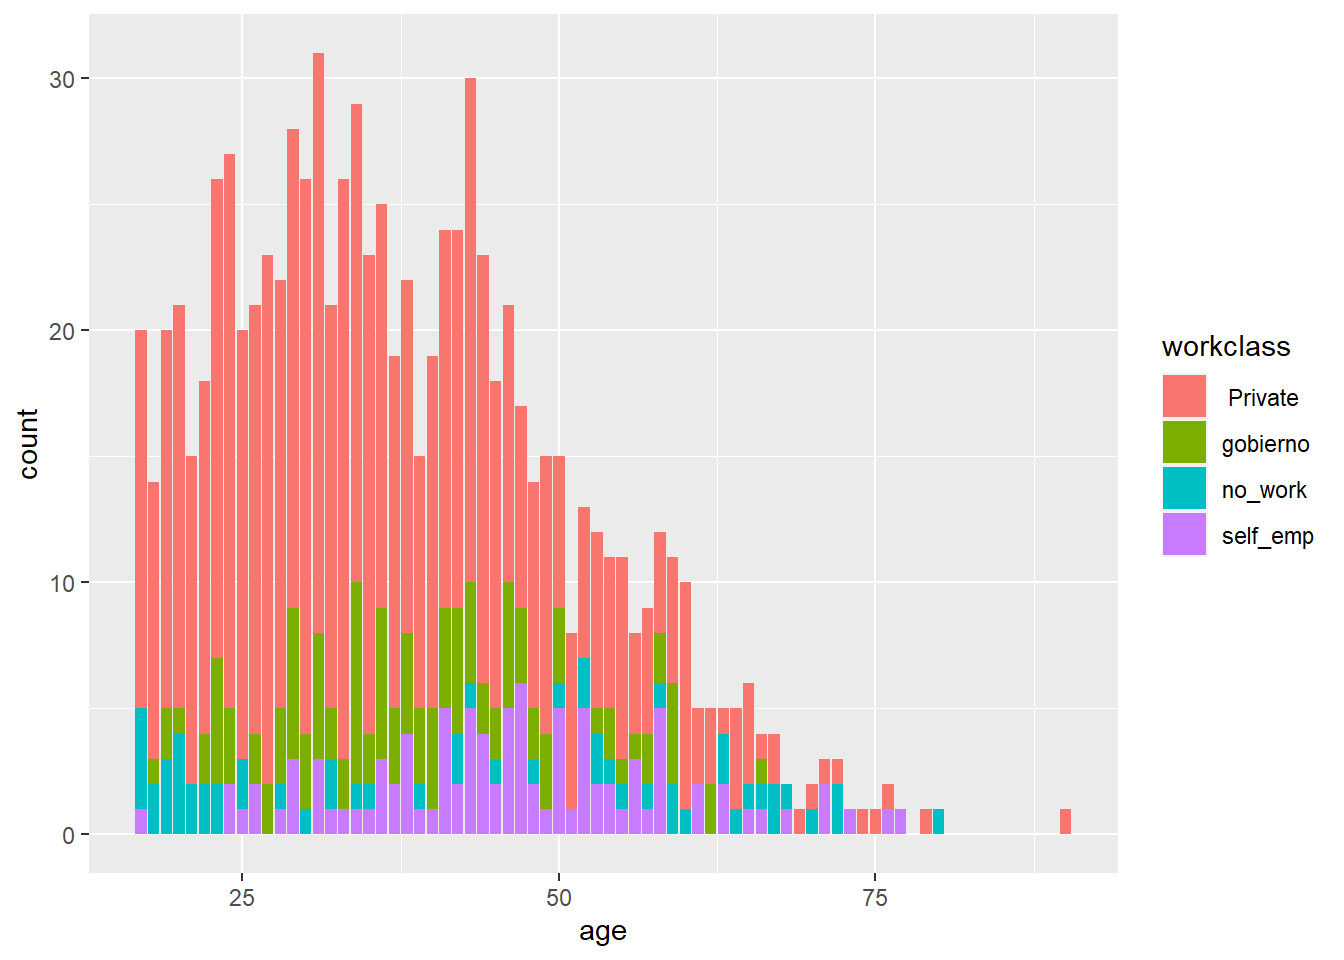
\includegraphics{pra01_Raquel_files/figure-latex/unnamed-chunk-22-1.pdf}
Vamos a ver ahora la matriz de porcentajes de frecuencias de Age y
Workclass.

\begin{Shaded}
\begin{Highlighting}[]
\NormalTok{t\textless{}{-}}\KeywordTok{table}\NormalTok{(datosAdult[}\DecValTok{1}\OperatorTok{:}\NormalTok{filas,]}\OperatorTok{$}\NormalTok{age,datosAdult[}\DecValTok{1}\OperatorTok{:}\NormalTok{filas,]}\OperatorTok{$}\NormalTok{workclass)}
\ControlFlowTok{for}\NormalTok{ (i }\ControlFlowTok{in} \DecValTok{1}\OperatorTok{:}\KeywordTok{dim}\NormalTok{(t)[}\DecValTok{1}\NormalTok{])\{}
\NormalTok{    t[i,]\textless{}{-}}\KeywordTok{round}\NormalTok{(t[i,]}\OperatorTok{/}\KeywordTok{sum}\NormalTok{(t[i,])}\OperatorTok{*}\DecValTok{100}\NormalTok{,}\DecValTok{2}\NormalTok{)}
\NormalTok{\}}
\NormalTok{t}
\end{Highlighting}
\end{Shaded}

\begin{verbatim}
##     
##       Private gobierno no_work self_emp
##   17    75.00     0.00   20.00     5.00
##   18    78.57     7.14   14.29     0.00
##   19    75.00    10.00   15.00     0.00
##   20    76.19     4.76   19.05     0.00
##   21    86.67     0.00   13.33     0.00
##   22    77.78    11.11   11.11     0.00
##   23    73.08    19.23    7.69     0.00
##   24    81.48    11.11    0.00     7.41
##   25    85.00     0.00   10.00     5.00
##   26    80.95     9.52    0.00     9.52
##   27    91.30     8.70    0.00     0.00
##   28    77.27    13.64    4.55     4.55
##   29    67.86    21.43    0.00    10.71
##   30    84.62    11.54    3.85     0.00
##   31    74.19    16.13    0.00     9.68
##   32    76.19     9.52    9.52     4.76
##   33    88.46     7.69    0.00     3.85
##   34    65.52    27.59    3.45     3.45
##   35    82.61     8.70    4.35     4.35
##   36    64.00    24.00    0.00    12.00
##   37    73.68    15.79    0.00    10.53
##   38    63.64    18.18    0.00    18.18
##   39    66.67    20.00    6.67     6.67
##   40    73.68    21.05    0.00     5.26
##   41    62.50    16.67    0.00    20.83
##   42    62.50    20.83    8.33     8.33
##   43    66.67    13.33    3.33    16.67
##   44    73.91     8.70    0.00    17.39
##   45    72.22    11.11    5.56    11.11
##   46    52.38    23.81    0.00    23.81
##   47    47.06    17.65    0.00    35.29
##   48    64.29    14.29    7.14    14.29
##   49    73.33    20.00    0.00     6.67
##   50    40.00    20.00    6.67    33.33
##   51    87.50     0.00    0.00    12.50
##   52    46.15     0.00   15.38    38.46
##   53    58.33     8.33   16.67    16.67
##   54    54.55    18.18    9.09    18.18
##   55    72.73     9.09    9.09     9.09
##   56    50.00    12.50    0.00    37.50
##   57    55.56    22.22   11.11    11.11
##   58    33.33    16.67    8.33    41.67
##   59    45.45    36.36   18.18     0.00
##   60    90.00     0.00   10.00     0.00
##   61    60.00     0.00    0.00    40.00
##   62    60.00    40.00    0.00     0.00
##   63    20.00     0.00   40.00    40.00
##   64    80.00     0.00   20.00     0.00
##   65    66.67     0.00   16.67    16.67
##   66    25.00    25.00   25.00    25.00
##   67    50.00     0.00   50.00     0.00
##   68     0.00     0.00   50.00    50.00
##   69   100.00     0.00    0.00     0.00
##   70    50.00     0.00   50.00     0.00
##   71    33.33     0.00    0.00    66.67
##   72    33.33     0.00   66.67     0.00
##   73     0.00     0.00    0.00   100.00
##   74   100.00     0.00    0.00     0.00
##   75   100.00     0.00    0.00     0.00
##   76    50.00     0.00    0.00    50.00
##   77     0.00     0.00    0.00   100.00
##   79   100.00     0.00    0.00     0.00
##   80     0.00     0.00  100.00     0.00
##   90   100.00     0.00    0.00     0.00
\end{verbatim}

\hypertarget{fnlgt}{%
\subsubsection{fnlgt}\label{fnlgt}}

Esta variable es el final weght, es decir, el número de personas que el
censo estima que representa. Esta variable sería interesante a la hora
de ver el peso real de una observación.

\begin{Shaded}
\begin{Highlighting}[]
\KeywordTok{summary}\NormalTok{(datosAdult}\OperatorTok{$}\NormalTok{fnlwgt)}
\end{Highlighting}
\end{Shaded}

\begin{verbatim}
##    Min. 1st Qu.  Median    Mean 3rd Qu.    Max. 
##   12285  117827  178356  189778  237051 1484705
\end{verbatim}

Vemos que la media representación es de 189.778 pero que el mínimo es
12.285 y el máximo 1.484.705, por lo que hay observaciones cuyo peso es
muy superior al de otras.

También vemos que la mediana es 178.356, que el Q1 es 117.827 y el Q3
237.051. El rango intercuantílico es 119.224. Teniendo en cuenta que un
valor atípico extremo es aquel que dista 3 veces el rango
intercuantílico por debajo de Q1 o por encima de Q3; es decir, aquel que
esté por debajo o por encima de Q1 y Q3 respectivamente en 357.672.

Vamos a verlo visualmente.

\begin{Shaded}
\begin{Highlighting}[]
\KeywordTok{plot}\NormalTok{(}\DataTypeTok{x=}\NormalTok{ datosAdult}\OperatorTok{$}\NormalTok{fnlwgt, }\DataTypeTok{col =}\StringTok{"blue"}\NormalTok{)}
\end{Highlighting}
\end{Shaded}

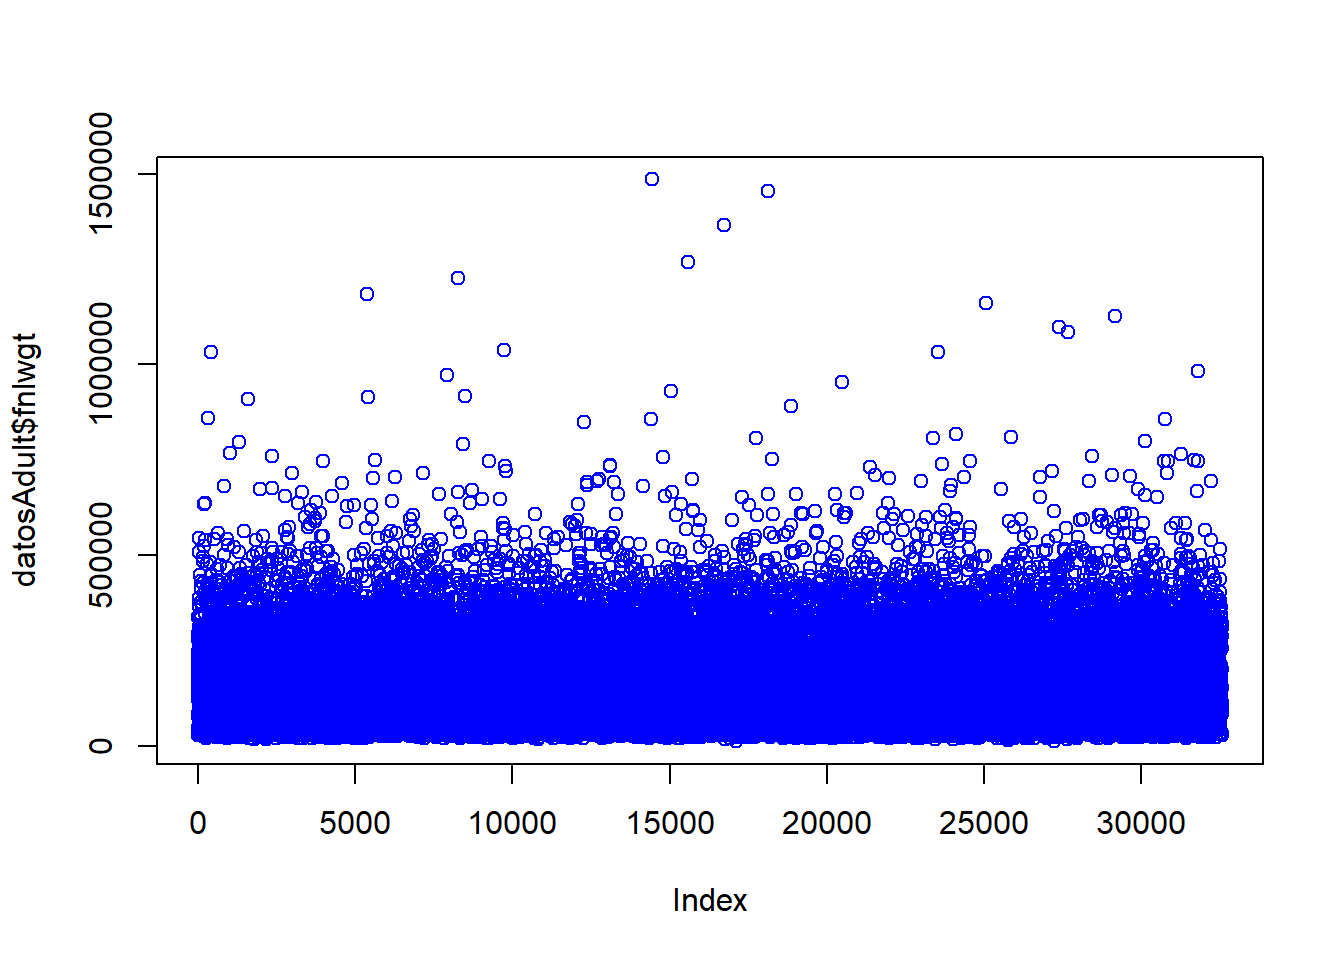
\includegraphics{pra01_Raquel_files/figure-latex/unnamed-chunk-25-1.pdf}
Con el gráfico vemos que hay outliers por arriba. Por abajo no porque
sería una cifra negativa y nuestro umbral mínimo es 0.

Vamos a ver también una caja de bigotes:

\begin{Shaded}
\begin{Highlighting}[]
\KeywordTok{boxplot}\NormalTok{(datosAdult}\OperatorTok{$}\NormalTok{fnlwgt,}
        \DataTypeTok{main =} \StringTok{"fnlwgt"}\NormalTok{,}
        \DataTypeTok{boxwex =} \FloatTok{0.5}\NormalTok{, }\DataTypeTok{col =} \StringTok{"red"}\NormalTok{)}
\end{Highlighting}
\end{Shaded}

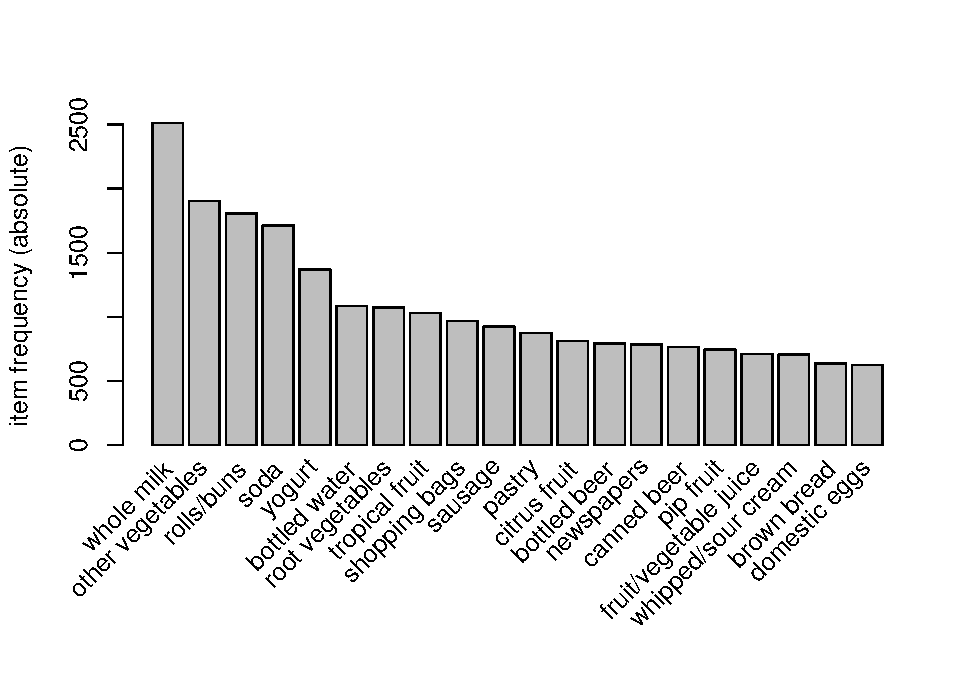
\includegraphics{pra01_Raquel_files/figure-latex/unnamed-chunk-26-1.pdf}

Calculamos por aquí el rango intercuantílico:

\begin{Shaded}
\begin{Highlighting}[]
\NormalTok{RIC=}\StringTok{ }\KeywordTok{quantile}\NormalTok{(datosAdult}\OperatorTok{$}\NormalTok{fnlwgt, }\DataTypeTok{prob=}\KeywordTok{c}\NormalTok{(}\FloatTok{0.25}\NormalTok{, }\FloatTok{0.75}\NormalTok{))}
\NormalTok{RIC}
\end{Highlighting}
\end{Shaded}

\begin{verbatim}
##    25%    75% 
## 117827 237051
\end{verbatim}

\begin{Shaded}
\begin{Highlighting}[]
\NormalTok{Valor\_outliers =}\StringTok{ }\NormalTok{(}\KeywordTok{quantile}\NormalTok{(datosAdult}\OperatorTok{$}\NormalTok{fnlwgt, }\DataTypeTok{prob=}\KeywordTok{c}\NormalTok{(}\FloatTok{0.75}\NormalTok{)) }\OperatorTok{{-}}\StringTok{ }\KeywordTok{quantile}\NormalTok{(datosAdult}\OperatorTok{$}\NormalTok{fnlwgt, }\DataTypeTok{prob=}\KeywordTok{c}\NormalTok{(}\FloatTok{0.25}\NormalTok{))) }\OperatorTok{*}\StringTok{ }\DecValTok{3}
\NormalTok{Valor\_outliers}
\end{Highlighting}
\end{Shaded}

\begin{verbatim}
##    75% 
## 357672
\end{verbatim}

Con lo cual vamos a ver cuántos son esos los valores por encima de esa
cantidad de la variable ya que nos desvirtúan el estudio y vemos si
podemos eliminarlos o los reemplazamos. Para ello creamos un df1
filtrando los datos que no serían outliers de fnlwgt.

\begin{Shaded}
\begin{Highlighting}[]
\NormalTok{df1 \textless{}{-}}\StringTok{ }\KeywordTok{filter}\NormalTok{(datosAdult, fnlwgt }\OperatorTok{\textless{}}\StringTok{ "357672"}\NormalTok{)}
\end{Highlighting}
\end{Shaded}

Y vemos la variable fnlwgt en nuestro dataframe filtrado gráficamente.

\begin{Shaded}
\begin{Highlighting}[]
\KeywordTok{boxplot}\NormalTok{(df1}\OperatorTok{$}\NormalTok{fnlwgt,}
        \DataTypeTok{main =} \StringTok{"fnlwgt"}\NormalTok{,}
        \DataTypeTok{boxwex =} \FloatTok{0.5}\NormalTok{, }\DataTypeTok{col =} \StringTok{"red"}\NormalTok{)}
\end{Highlighting}
\end{Shaded}

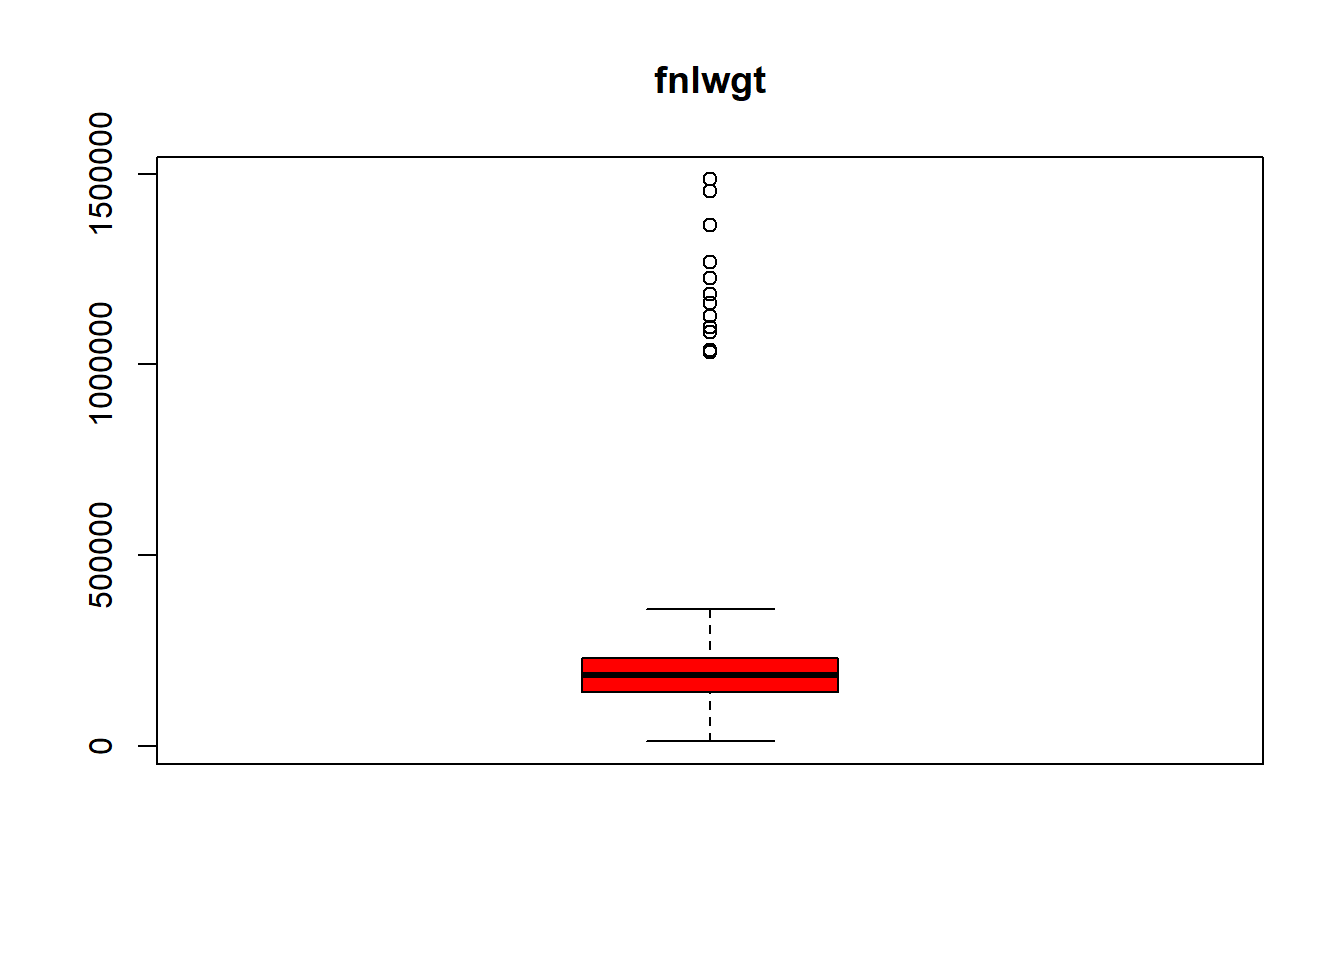
\includegraphics{pra01_Raquel_files/figure-latex/unnamed-chunk-30-1.pdf}

Vemos que sigue habiendo outliers pero serían valores atípicos leves ya
que los extremos los hemos eliminado en el dataframe df1.

\hypertarget{marital-status}{%
\subsubsection{Marital-status}\label{marital-status}}

Vamos a categorizar ahora la variable marital- status.

\begin{Shaded}
\begin{Highlighting}[]
\KeywordTok{table}\NormalTok{(df1}\OperatorTok{$}\StringTok{\textasciigrave{}}\DataTypeTok{marital{-}status}\StringTok{\textasciigrave{}}\NormalTok{)}
\end{Highlighting}
\end{Shaded}

\begin{verbatim}
## 
##               Divorced      Married-AF-spouse     Married-civ-spouse 
##                   3572                     16                  11985 
##  Married-spouse-absent          Never-married              Separated 
##                    335                   8448                    861 
##                Widowed 
##                    806
\end{verbatim}

\begin{Shaded}
\begin{Highlighting}[]
\NormalTok{casado \textless{}{-}}\StringTok{ }\KeywordTok{c}\NormalTok{(}\StringTok{" Married{-}AF{-}spouse"}\NormalTok{, }\StringTok{" Married{-}civ{-}spouse"}\NormalTok{, }\StringTok{"Married{-}spouse{-}absent"}\NormalTok{)}
\NormalTok{no.casado \textless{}{-}}\StringTok{ }\KeywordTok{c}\NormalTok{(}\StringTok{" Divorced"}\NormalTok{, }\StringTok{" Separated"}\NormalTok{, }\StringTok{" Widowed"}\NormalTok{)}
\NormalTok{nunca.casado \textless{}{-}}\StringTok{ }\KeywordTok{c}\NormalTok{(}\StringTok{" Never{-}married"}\NormalTok{)}
\end{Highlighting}
\end{Shaded}

Mediante una función cambiamos las categorías.

\begin{Shaded}
\begin{Highlighting}[]
\NormalTok{estado.civil \textless{}{-}}\StringTok{ }\ControlFlowTok{function}\NormalTok{(estado)\{}
  \ControlFlowTok{if}\NormalTok{(estado }\OperatorTok{\%in\%}\StringTok{ }\NormalTok{casado)\{}
    \KeywordTok{return}\NormalTok{(}\StringTok{"casado"}\NormalTok{)}
\NormalTok{  \}}\ControlFlowTok{else} \ControlFlowTok{if}\NormalTok{(estado }\OperatorTok{\%in\%}\StringTok{ }\NormalTok{no.casado)\{}
    \KeywordTok{return}\NormalTok{(}\StringTok{"no.casado"}\NormalTok{)}
\NormalTok{  \}}\ControlFlowTok{else}\NormalTok{\{}
    \KeywordTok{return}\NormalTok{(}\StringTok{"nunca.casado"}\NormalTok{)}
\NormalTok{  \}}
\NormalTok{\}}
\end{Highlighting}
\end{Shaded}

\begin{Shaded}
\begin{Highlighting}[]
\NormalTok{df1}\OperatorTok{$}\StringTok{\textasciigrave{}}\DataTypeTok{marital{-}status}\StringTok{\textasciigrave{}}\NormalTok{\textless{}{-}}\StringTok{ }\KeywordTok{sapply}\NormalTok{(df1}\OperatorTok{$}\StringTok{\textasciigrave{}}\DataTypeTok{marital{-}status}\StringTok{\textasciigrave{}}\NormalTok{, estado.civil)}
\end{Highlighting}
\end{Shaded}

Comprobamos de nuevo la variable.

\begin{Shaded}
\begin{Highlighting}[]
\KeywordTok{table}\NormalTok{(df1}\OperatorTok{$}\StringTok{\textasciigrave{}}\DataTypeTok{marital{-}status}\StringTok{\textasciigrave{}}\NormalTok{)}
\end{Highlighting}
\end{Shaded}

\begin{verbatim}
## 
##       casado    no.casado nunca.casado 
##        12001         5239         8783
\end{verbatim}

Vamos a verla gráficamente con edad.

\begin{Shaded}
\begin{Highlighting}[]
\KeywordTok{unique}\NormalTok{(df1}\OperatorTok{$}\StringTok{\textasciigrave{}}\DataTypeTok{marital{-}status}\StringTok{\textasciigrave{}}\NormalTok{)}
\end{Highlighting}
\end{Shaded}

\begin{verbatim}
## [1] "no.casado"    "casado"       "nunca.casado"
\end{verbatim}

\begin{Shaded}
\begin{Highlighting}[]
\KeywordTok{ggplot}\NormalTok{(}\DataTypeTok{data=}\NormalTok{df1[}\DecValTok{1}\OperatorTok{:}\NormalTok{filas,],}\KeywordTok{aes}\NormalTok{(}\DataTypeTok{x=}\NormalTok{age,}\DataTypeTok{fill=}\StringTok{\textasciigrave{}}\DataTypeTok{marital{-}status}\StringTok{\textasciigrave{}}\NormalTok{))}\OperatorTok{+}\KeywordTok{geom\_bar}\NormalTok{()}
\end{Highlighting}
\end{Shaded}

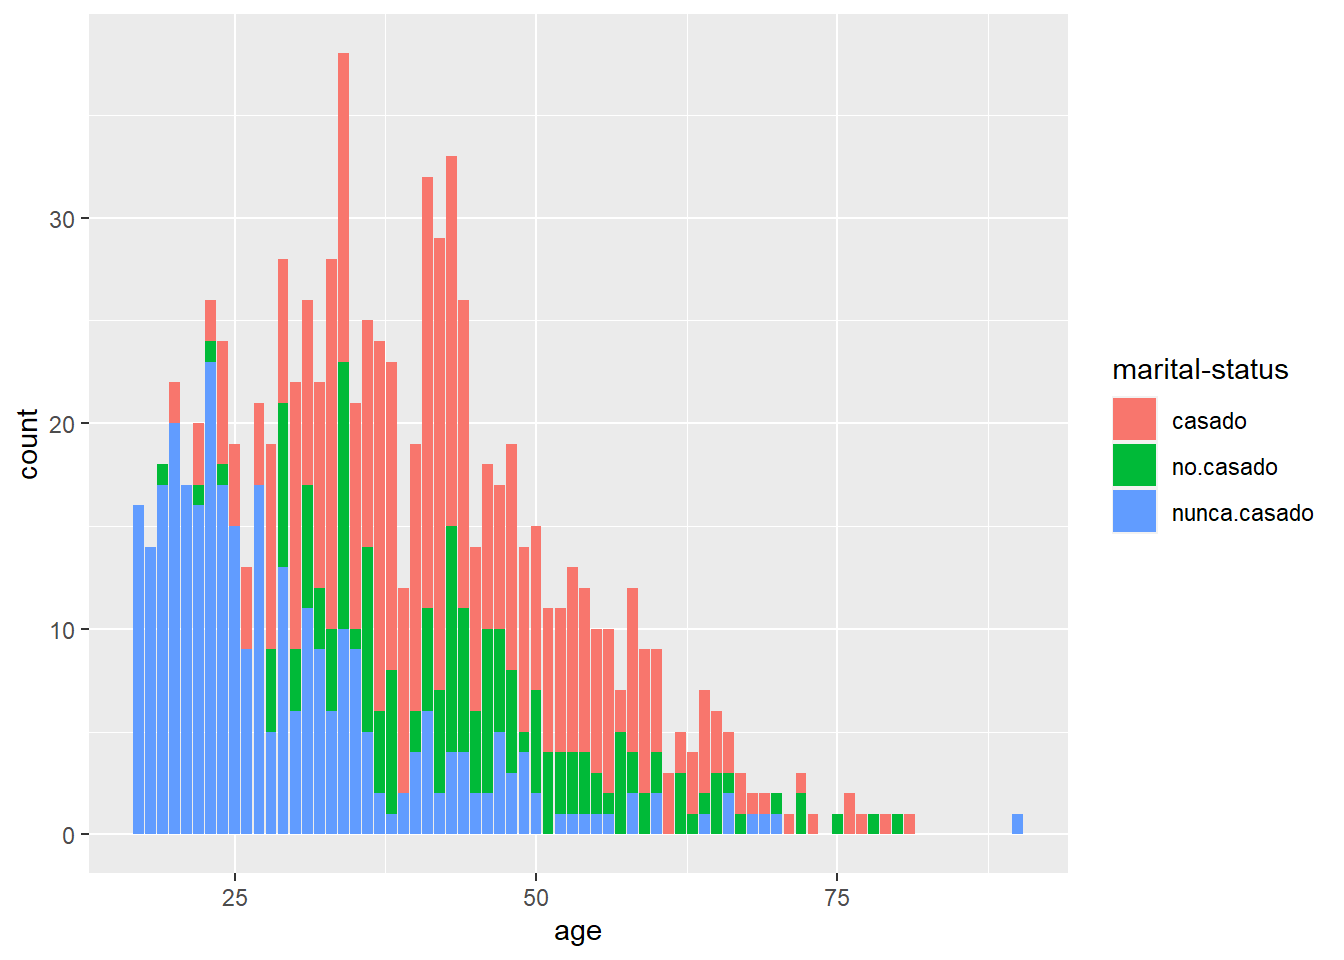
\includegraphics{pra01_Raquel_files/figure-latex/unnamed-chunk-37-1.pdf}

Y por sexo:

\begin{Shaded}
\begin{Highlighting}[]
\KeywordTok{ggplot}\NormalTok{(}\DataTypeTok{data=}\NormalTok{df1[}\DecValTok{1}\OperatorTok{:}\NormalTok{filas,],}\KeywordTok{aes}\NormalTok{(}\DataTypeTok{x=}\NormalTok{sex,}\DataTypeTok{fill=}\StringTok{\textasciigrave{}}\DataTypeTok{marital{-}status}\StringTok{\textasciigrave{}}\NormalTok{))}\OperatorTok{+}\KeywordTok{geom\_bar}\NormalTok{()}
\end{Highlighting}
\end{Shaded}

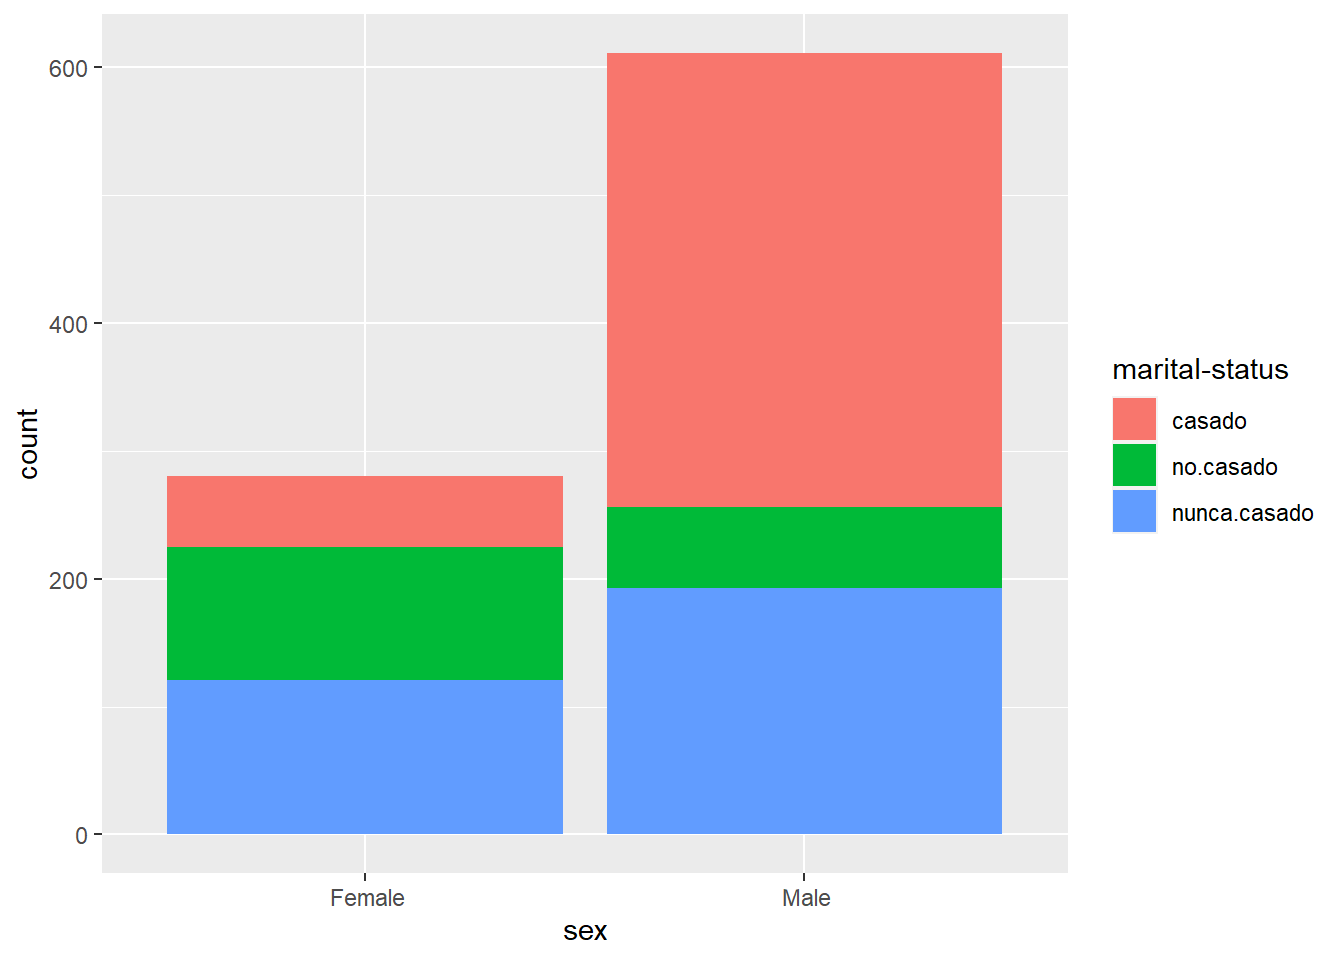
\includegraphics{pra01_Raquel_files/figure-latex/unnamed-chunk-38-1.pdf}

\hypertarget{occupation}{%
\subsubsection{Occupation}\label{occupation}}

Vamos a categorizar la variable occupation

\begin{Shaded}
\begin{Highlighting}[]
\KeywordTok{unique}\NormalTok{(df1}\OperatorTok{$}\NormalTok{occupation)}
\end{Highlighting}
\end{Shaded}

\begin{verbatim}
##  [1] " Handlers-cleaners" " Prof-specialty"    " Exec-managerial"  
##  [4] " Other-service"     " Adm-clerical"      " Sales"            
##  [7] " Craft-repair"      " Transport-moving"  " Farming-fishing"  
## [10] " Machine-op-inspct" " Tech-support"      " ?"                
## [13] " Protective-serv"   " Armed-Forces"      " Priv-house-serv"
\end{verbatim}

Hay datos de origen desconocido. Vamos a ver la tabla de frecuencias.

\begin{Shaded}
\begin{Highlighting}[]
\KeywordTok{table}\NormalTok{(df1}\OperatorTok{$}\NormalTok{occupation)}
\end{Highlighting}
\end{Shaded}

\begin{verbatim}
## 
##                  ?       Adm-clerical       Armed-Forces 
##               1456               3043                  8 
##       Craft-repair    Exec-managerial    Farming-fishing 
##               3253               3261                717 
##  Handlers-cleaners  Machine-op-inspct      Other-service 
##               1104               1667               2589 
##    Priv-house-serv     Prof-specialty    Protective-serv 
##                115               3311                542 
##              Sales       Tech-support   Transport-moving 
##               2941                740               1276
\end{verbatim}

Hay 1456 profesiones de orgien desconocido. También vemos que hay 8 que
pertenecen a las fuerzas armadas, que vamos a unir con los de origen
desconocido.

\begin{Shaded}
\begin{Highlighting}[]
\NormalTok{White\_collar \textless{}{-}}\StringTok{ }\KeywordTok{c}\NormalTok{(}\StringTok{" Adm{-}clerical"}\NormalTok{, }\StringTok{" Exec{-}managerial"}\NormalTok{, }\StringTok{" Tech{-}support"}\NormalTok{)}
\NormalTok{Desconocido \textless{}{-}}\StringTok{ }\KeywordTok{c}\NormalTok{(}\StringTok{" Armed{-}Forces"}\NormalTok{, }\StringTok{" Unknown"}\NormalTok{)}
\NormalTok{Blue\_collar \textless{}{-}}\StringTok{ }\KeywordTok{c}\NormalTok{(}\StringTok{" Craft{-}repair"}\NormalTok{, }\StringTok{" Farming{-}fishing"}\NormalTok{, }\StringTok{" Handlers{-}cleaners"}\NormalTok{, }\StringTok{" Machine{-}op{-}inspct"}\NormalTok{, }\StringTok{" Transport{-}moving"}\NormalTok{)}
\NormalTok{Servicios \textless{}{-}}\StringTok{ }\KeywordTok{c}\NormalTok{(}\StringTok{" Other{-}service"}\NormalTok{, }\StringTok{" Priv{-}house{-}serv"}\NormalTok{)}
\NormalTok{Profesional \textless{}{-}}\StringTok{ }\KeywordTok{c}\NormalTok{(}\StringTok{" Prof{-}specialty"}\NormalTok{)}
\NormalTok{Ventas \textless{}{-}}\StringTok{ }\KeywordTok{c}\NormalTok{(}\StringTok{" Sales"}\NormalTok{)}
\end{Highlighting}
\end{Shaded}

\begin{Shaded}
\begin{Highlighting}[]
\NormalTok{ocupaciones \textless{}{-}}\StringTok{ }\ControlFlowTok{function}\NormalTok{(ocupacion)\{}
  \ControlFlowTok{if}\NormalTok{(ocupacion }\OperatorTok{\%in\%}\StringTok{ }\NormalTok{White\_collar)\{}
    \KeywordTok{return}\NormalTok{(}\StringTok{"White\_collar"}\NormalTok{)}
\NormalTok{  \}}\ControlFlowTok{else} \ControlFlowTok{if}\NormalTok{(ocupacion }\OperatorTok{\%in\%}\StringTok{ }\NormalTok{Ventas)\{}
    \KeywordTok{return}\NormalTok{(}\StringTok{"Sales"}\NormalTok{)}
\NormalTok{  \}}\ControlFlowTok{else} \ControlFlowTok{if}\NormalTok{(ocupacion }\OperatorTok{\%in\%}\StringTok{ }\NormalTok{Blue\_collar)\{}
    \KeywordTok{return}\NormalTok{(}\StringTok{"Blue\_collar"}\NormalTok{)}
\NormalTok{  \}}\ControlFlowTok{else} \ControlFlowTok{if}\NormalTok{(ocupacion }\OperatorTok{\%in\%}\StringTok{ }\NormalTok{Servicios)\{}
    \KeywordTok{return}\NormalTok{(}\StringTok{"Servicios"}\NormalTok{)}
\NormalTok{  \}}\ControlFlowTok{else} \ControlFlowTok{if}\NormalTok{(ocupacion }\OperatorTok{\%in\%}\StringTok{ }\NormalTok{Profesional)\{}
    \KeywordTok{return}\NormalTok{(}\StringTok{"Profesional"}\NormalTok{)}
\NormalTok{  \}}\ControlFlowTok{else}\NormalTok{\{}\KeywordTok{return}\NormalTok{(}\StringTok{"Desconocido"}\NormalTok{)\}}
\NormalTok{\}}
\end{Highlighting}
\end{Shaded}

\begin{Shaded}
\begin{Highlighting}[]
\NormalTok{df1}\OperatorTok{$}\NormalTok{occupation\textless{}{-}}\StringTok{ }\KeywordTok{sapply}\NormalTok{(df1}\OperatorTok{$}\NormalTok{occupation, ocupaciones)}
\end{Highlighting}
\end{Shaded}

\begin{Shaded}
\begin{Highlighting}[]
\KeywordTok{table}\NormalTok{(df1}\OperatorTok{$}\NormalTok{occupation)}
\end{Highlighting}
\end{Shaded}

\begin{verbatim}
## 
##  Blue_collar  Desconocido  Profesional        Sales    Servicios 
##         8017         2006         3311         2941         2704 
## White_collar 
##         7044
\end{verbatim}

Ya tenemos categorizada nuestra variable. Vamos a ver gráficamente la
relación entre edad y la ocupación,

\begin{Shaded}
\begin{Highlighting}[]
\KeywordTok{ggplot}\NormalTok{(}\DataTypeTok{data=}\NormalTok{df1[}\DecValTok{1}\OperatorTok{:}\NormalTok{filas,],}\KeywordTok{aes}\NormalTok{(}\DataTypeTok{x=}\NormalTok{age,}\DataTypeTok{fill=}\NormalTok{occupation))}\OperatorTok{+}\KeywordTok{geom\_bar}\NormalTok{()}
\end{Highlighting}
\end{Shaded}

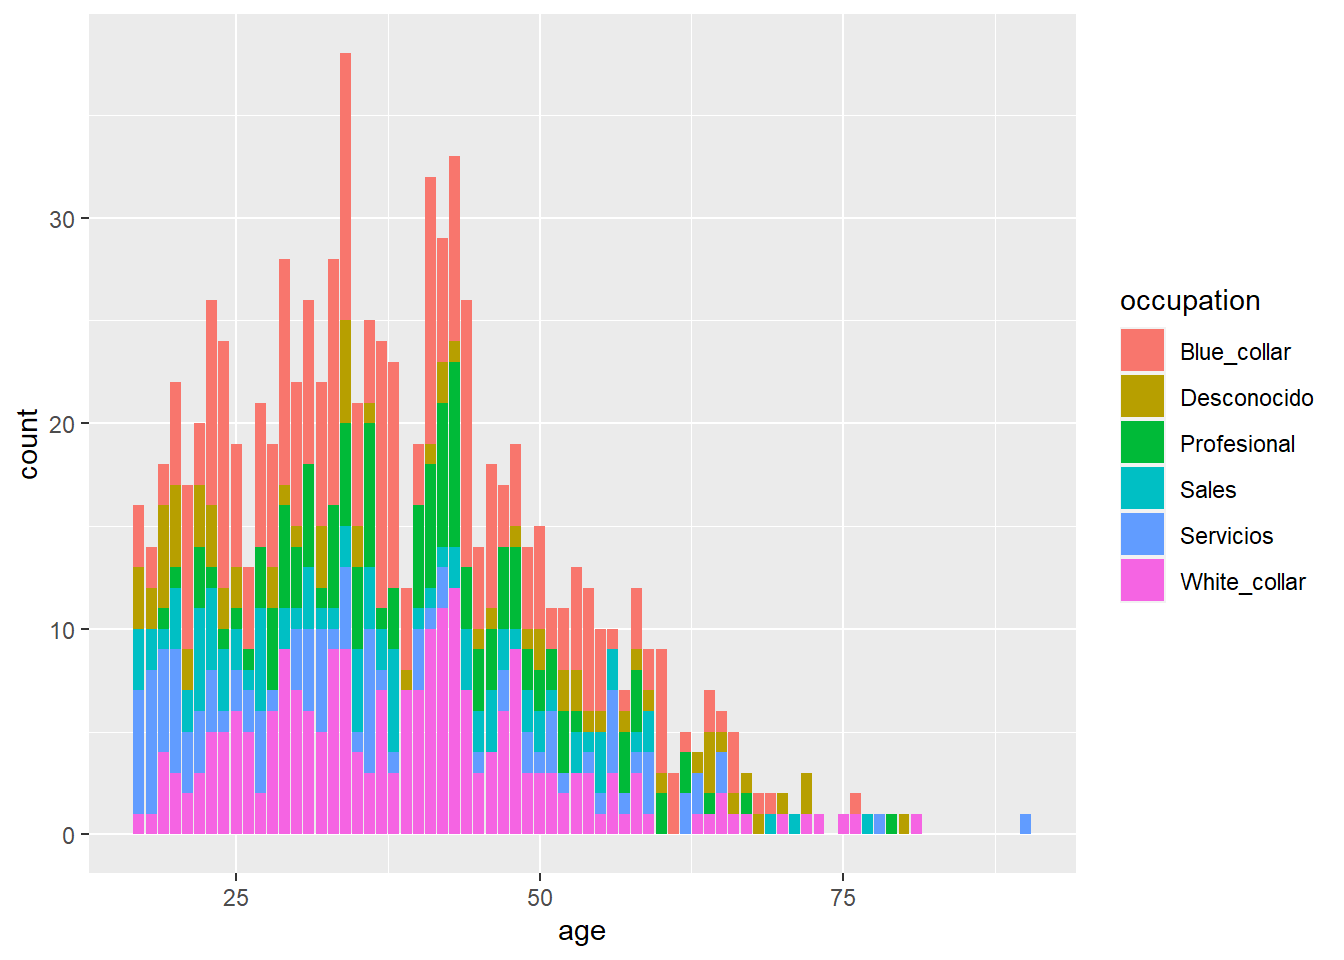
\includegraphics{pra01_Raquel_files/figure-latex/unnamed-chunk-45-1.pdf}

Y por sexo.

\begin{Shaded}
\begin{Highlighting}[]
\KeywordTok{ggplot}\NormalTok{(}\DataTypeTok{data=}\NormalTok{df1[}\DecValTok{1}\OperatorTok{:}\NormalTok{filas,],}\KeywordTok{aes}\NormalTok{(}\DataTypeTok{x=}\NormalTok{sex,}\DataTypeTok{fill=}\StringTok{\textasciigrave{}}\DataTypeTok{marital{-}status}\StringTok{\textasciigrave{}}\NormalTok{))}\OperatorTok{+}\KeywordTok{geom\_bar}\NormalTok{()}
\end{Highlighting}
\end{Shaded}

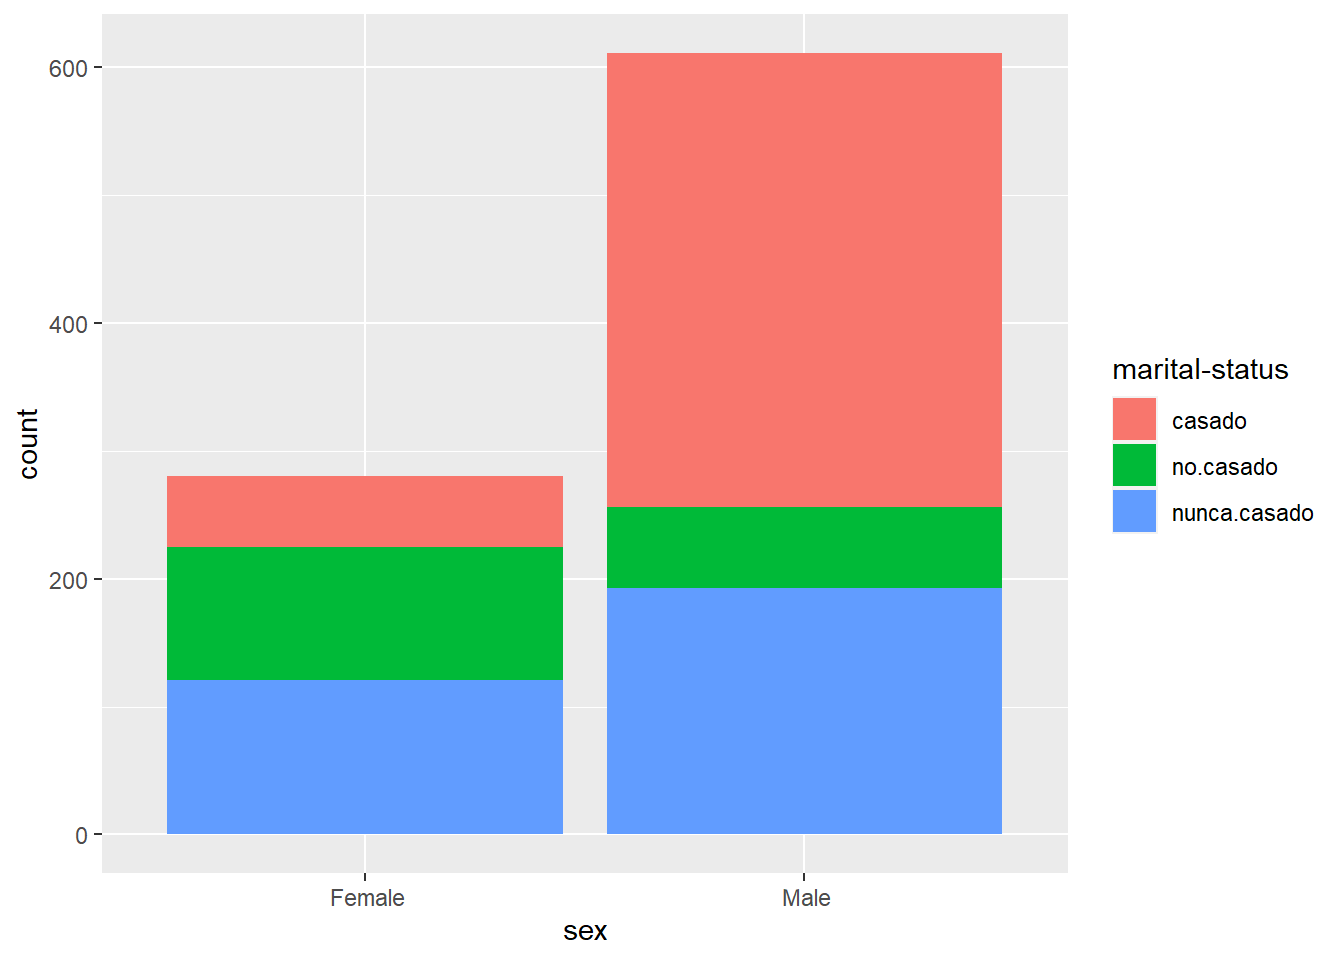
\includegraphics{pra01_Raquel_files/figure-latex/unnamed-chunk-46-1.pdf}
Vamos a ver también la relación entre ocupación y workclass.

\begin{Shaded}
\begin{Highlighting}[]
\KeywordTok{ggplot}\NormalTok{(}\DataTypeTok{data=}\NormalTok{df1[}\DecValTok{1}\OperatorTok{:}\NormalTok{filas,],}\KeywordTok{aes}\NormalTok{(}\DataTypeTok{x=}\NormalTok{occupation,}\DataTypeTok{fill=}\NormalTok{workclass))}\OperatorTok{+}\KeywordTok{geom\_bar}\NormalTok{()}
\end{Highlighting}
\end{Shaded}

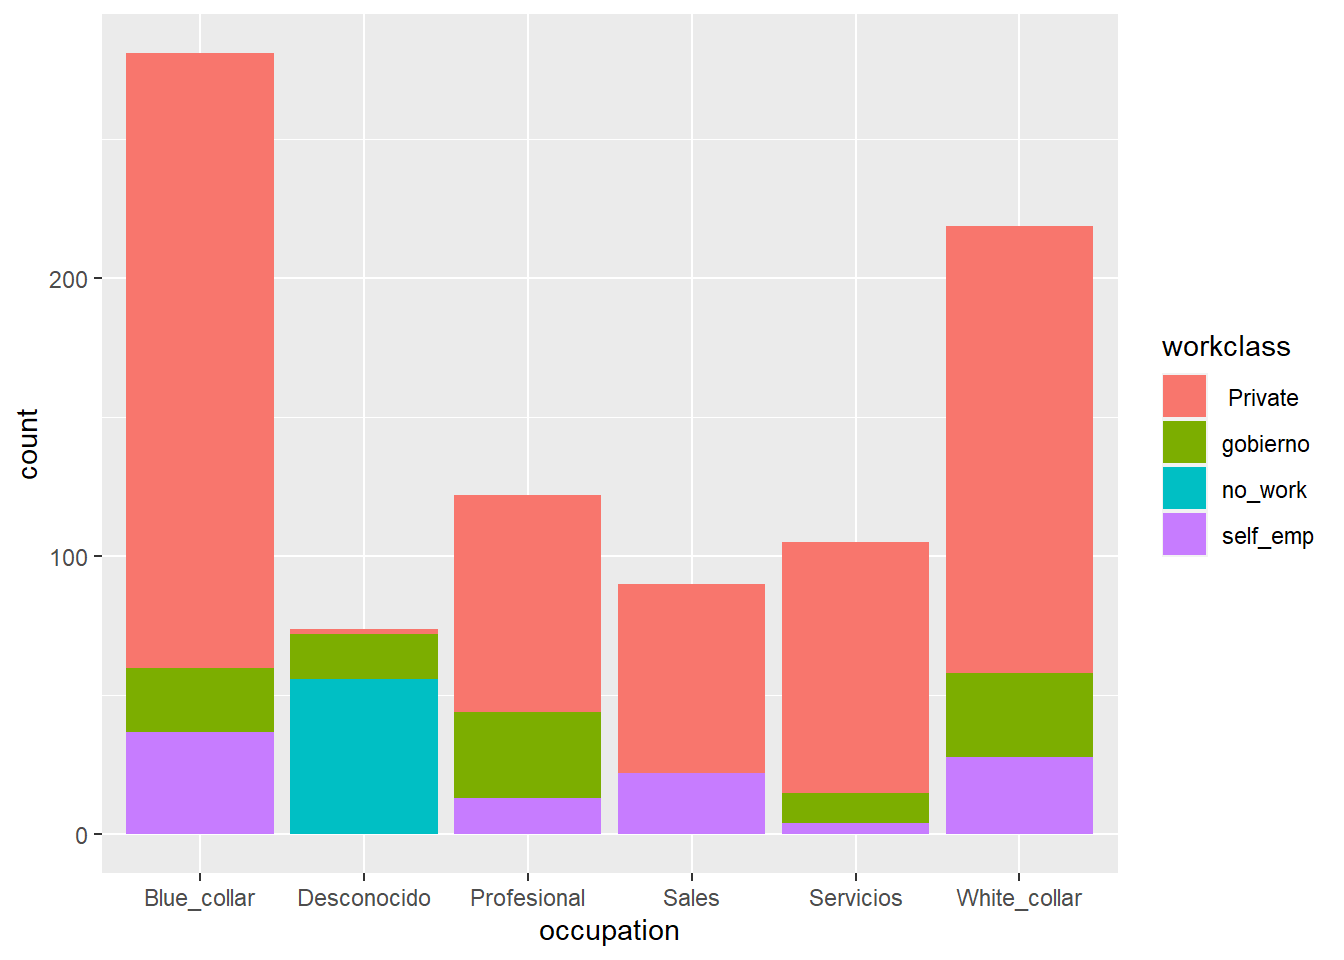
\includegraphics{pra01_Raquel_files/figure-latex/unnamed-chunk-47-1.pdf}

Vemos que la mayoría de blue collar trabajan para la empresa privada,
seguidos de autónomos y por último una pequeña cantidad trabaja para el
gobierno. De origen desconocido la mayoría no trabajan, teniendo en
cuenta que hemos incluido aquí una gran cantidad de datos de los que no
sabíamos de dónde salían es importante ver que realmente es gente que en
su mayoría no tiene trabajo. Con respecto a las ventas vemos que o son
autónomos o trabajan en el sector privado, pero no trabajan para el
gobierno ni están sin empleo. En el sector servicios hay una pequeña
cantidad de trabajadores autónomos, algunos trabajan para el gobierno y
la mayoría lo hacen en el sector privado. Y los white collars trabajan
principalmente en el sector privado, y aparentemente la misma canditdad
trabaja para el gobierno o es autonoma, pero tampoco están desempleados.

\hypertarget{native-country}{%
\subsubsection{native country}\label{native-country}}

Vamos a ver los paises y a categorizar la variable

\begin{Shaded}
\begin{Highlighting}[]
\KeywordTok{unique}\NormalTok{(df1}\OperatorTok{$}\StringTok{\textasciigrave{}}\DataTypeTok{native{-}country}\StringTok{\textasciigrave{}}\NormalTok{)}
\end{Highlighting}
\end{Shaded}

\begin{verbatim}
##  [1] " United-States"              " Cuba"                      
##  [3] " Jamaica"                    " India"                     
##  [5] " ?"                          " Mexico"                    
##  [7] " South"                      " Puerto-Rico"               
##  [9] " England"                    " Canada"                    
## [11] " Iran"                       " Philippines"               
## [13] " Italy"                      " Poland"                    
## [15] " Columbia"                   " Cambodia"                  
## [17] " Thailand"                   " Germany"                   
## [19] " Ecuador"                    " Laos"                      
## [21] " Taiwan"                     " Haiti"                     
## [23] " Portugal"                   " Dominican-Republic"        
## [25] " France"                     " El-Salvador"               
## [27] " Guatemala"                  " China"                     
## [29] " Japan"                      " Yugoslavia"                
## [31] " Peru"                       " Outlying-US(Guam-USVI-etc)"
## [33] " Greece"                     " Nicaragua"                 
## [35] " Honduras"                   " Vietnam"                   
## [37] " Trinadad&Tobago"            " Hong"                      
## [39] " Ireland"                    " Scotland"                  
## [41] " Hungary"                    " Holand-Netherlands"
\end{verbatim}

\begin{Shaded}
\begin{Highlighting}[]
\KeywordTok{boxplot}\NormalTok{(df1}\OperatorTok{$}\NormalTok{fnlwgt,}
        \DataTypeTok{main =} \StringTok{"native{-}country"}\NormalTok{,}
        \DataTypeTok{boxwex =} \FloatTok{0.5}\NormalTok{, }\DataTypeTok{col =} \StringTok{"red"}\NormalTok{)}
\end{Highlighting}
\end{Shaded}

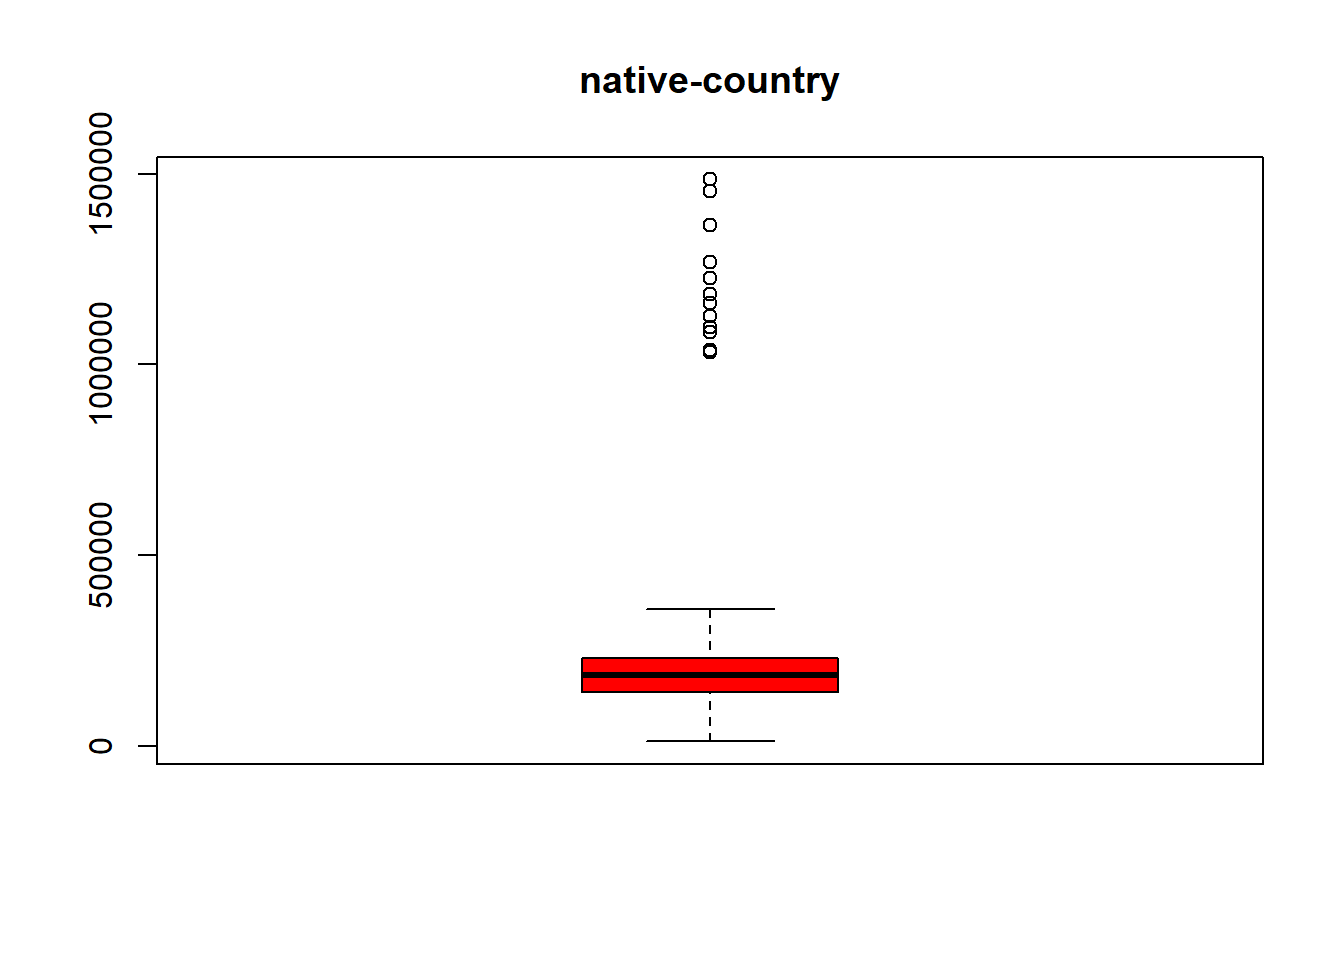
\includegraphics{pra01_Raquel_files/figure-latex/unnamed-chunk-49-1.pdf}
Vemos que hay algunos datos outliers. Vamos a ver la tabla de
frecuencias y creamos las distintas categorías, así veremos si sigue
habiendo outliers o no.

\begin{Shaded}
\begin{Highlighting}[]
\KeywordTok{table}\NormalTok{(df1}\OperatorTok{$}\StringTok{\textasciigrave{}}\DataTypeTok{native{-}country}\StringTok{\textasciigrave{}}\NormalTok{)}
\end{Highlighting}
\end{Shaded}

\begin{verbatim}
## 
##                           ?                    Cambodia 
##                         489                          16 
##                      Canada                       China 
##                          88                          59 
##                    Columbia                        Cuba 
##                          53                          92 
##          Dominican-Republic                     Ecuador 
##                          66                          28 
##                 El-Salvador                     England 
##                          75                          68 
##                      France                     Germany 
##                          22                         105 
##                      Greece                   Guatemala 
##                          26                          48 
##                       Haiti          Holand-Netherlands 
##                          43                           1 
##                    Honduras                        Hong 
##                          10                          20 
##                     Hungary                       India 
##                          12                          85 
##                        Iran                     Ireland 
##                          36                          20 
##                       Italy                     Jamaica 
##                          64                          75 
##                       Japan                        Laos 
##                          43                          15 
##                      Mexico                   Nicaragua 
##                         454                          26 
##  Outlying-US(Guam-USVI-etc)                        Peru 
##                          11                          24 
##                 Philippines                      Poland 
##                         143                          56 
##                    Portugal                 Puerto-Rico 
##                          24                         106 
##                    Scotland                       South 
##                           9                          69 
##                      Taiwan                    Thailand 
##                          47                          16 
##             Trinadad&Tobago               United-States 
##                          16                       23292 
##                     Vietnam                  Yugoslavia 
##                          57                          14
\end{verbatim}

\begin{Shaded}
\begin{Highlighting}[]
\NormalTok{Asia \textless{}{-}}\StringTok{ }\KeywordTok{c}\NormalTok{(}\StringTok{" Cambodia"}\NormalTok{, }\StringTok{" China"}\NormalTok{, }\StringTok{" Hong"}\NormalTok{, }\StringTok{" India"}\NormalTok{, }\StringTok{" Iran"}\NormalTok{, }\StringTok{" Japan"}\NormalTok{, }\StringTok{" Laos"}\NormalTok{, }\StringTok{" Philippines"}\NormalTok{, }\StringTok{" Taiwan"}\NormalTok{, }\StringTok{" Thailand"}\NormalTok{, }\StringTok{" Vietnam"}\NormalTok{)}
\NormalTok{Nor\_America \textless{}{-}}\StringTok{ }\KeywordTok{c}\NormalTok{(}\StringTok{" Canada"}\NormalTok{, }\StringTok{" United{-}States"}\NormalTok{)}
\NormalTok{Sur\_America \textless{}{-}}\StringTok{ }\KeywordTok{c}\NormalTok{(}\StringTok{" Columbia"}\NormalTok{, }\StringTok{" Cuba"}\NormalTok{, }\StringTok{" Dominican{-}Republic"}\NormalTok{, }\StringTok{" Ecuador"}\NormalTok{, }\StringTok{" El{-}Salvador"}\NormalTok{, }\StringTok{" Guatemala"}\NormalTok{, }\StringTok{" Haiti"}\NormalTok{, }\StringTok{" Honduras"}\NormalTok{, }\StringTok{" Jamaica"}\NormalTok{, }\StringTok{" Mexico"}\NormalTok{, }\StringTok{" Nicaragua"}\NormalTok{, }\StringTok{" Outlying{-}US(Guam{-}USVI{-}etc"}\NormalTok{, }\StringTok{" Peru"}\NormalTok{, }\StringTok{" Puerto{-}Rico"}\NormalTok{, }\StringTok{" Trinidad\&Tobago"}\NormalTok{)}
\NormalTok{Europa \textless{}{-}}\KeywordTok{c}\NormalTok{(}\StringTok{" England"}\NormalTok{, }\StringTok{" France"}\NormalTok{, }\StringTok{" Germany"}\NormalTok{, }\StringTok{" Greece"}\NormalTok{, }\StringTok{" Holand{-}Netherlands"}\NormalTok{, }\StringTok{" Hungary"}\NormalTok{, }\StringTok{" Ireland"}\NormalTok{, }\StringTok{" Italy"}\NormalTok{, }\StringTok{" Poland"}\NormalTok{, }\StringTok{" Portugal"}\NormalTok{, }\StringTok{" Scotland"}\NormalTok{, }\StringTok{" Yugoslavia"}\NormalTok{)}
\NormalTok{Otros \textless{}{-}}\StringTok{ }\KeywordTok{c}\NormalTok{(}\StringTok{" South"}\NormalTok{, }\StringTok{" ?"}\NormalTok{)}
\end{Highlighting}
\end{Shaded}

\begin{Shaded}
\begin{Highlighting}[]
\NormalTok{continente \textless{}{-}}\ControlFlowTok{function}\NormalTok{(pais)\{}
    \ControlFlowTok{if}\NormalTok{(pais }\OperatorTok{\%in\%}\StringTok{ }\NormalTok{Asia)\{}
      \KeywordTok{return}\NormalTok{(}\StringTok{"Asia"}\NormalTok{)}
\NormalTok{    \}}\ControlFlowTok{else} \ControlFlowTok{if}\NormalTok{(pais }\OperatorTok{\%in\%}\StringTok{ }\NormalTok{Nor\_America)\{}
      \KeywordTok{return}\NormalTok{(}\StringTok{"Nor\_America"}\NormalTok{)}
\NormalTok{    \}}\ControlFlowTok{else} \ControlFlowTok{if}\NormalTok{(pais }\OperatorTok{\%in\%}\StringTok{ }\NormalTok{Sur\_America)\{}
      \KeywordTok{return}\NormalTok{(}\StringTok{"Sur\_America"}\NormalTok{)}
\NormalTok{    \}}\ControlFlowTok{else} \ControlFlowTok{if}\NormalTok{(pais }\OperatorTok{\%in\%}\StringTok{ }\NormalTok{Europa)\{}
      \KeywordTok{return}\NormalTok{(}\StringTok{"Europa"}\NormalTok{)}
\NormalTok{    \}}\ControlFlowTok{else}\NormalTok{\{}
      \KeywordTok{return}\NormalTok{(}\StringTok{"Otros"}\NormalTok{)}
\NormalTok{    \}}
\NormalTok{\}}
\end{Highlighting}
\end{Shaded}

\begin{Shaded}
\begin{Highlighting}[]
\NormalTok{df1}\OperatorTok{$}\StringTok{\textasciigrave{}}\DataTypeTok{native{-}country}\StringTok{\textasciigrave{}}\NormalTok{\textless{}{-}}\StringTok{ }\KeywordTok{sapply}\NormalTok{(df1}\OperatorTok{$}\StringTok{\textasciigrave{}}\DataTypeTok{native{-}country}\StringTok{\textasciigrave{}}\NormalTok{, continente)}
\end{Highlighting}
\end{Shaded}

Volvemos a ver la tabla de frecuencias y la caja de bigotes.

\begin{Shaded}
\begin{Highlighting}[]
\KeywordTok{table}\NormalTok{(df1}\OperatorTok{$}\StringTok{\textasciigrave{}}\DataTypeTok{native{-}country}\StringTok{\textasciigrave{}}\NormalTok{)}
\end{Highlighting}
\end{Shaded}

\begin{verbatim}
## 
##        Asia      Europa Nor_America       Otros Sur_America 
##         537         421       23380         585        1100
\end{verbatim}

\begin{Shaded}
\begin{Highlighting}[]
\KeywordTok{boxplot}\NormalTok{(df1}\OperatorTok{$}\NormalTok{fnlwgt,}
        \DataTypeTok{main =} \StringTok{"native{-}country"}\NormalTok{,}
        \DataTypeTok{boxwex =} \FloatTok{0.5}\NormalTok{, }\DataTypeTok{col =} \StringTok{"blue"}\NormalTok{)}
\end{Highlighting}
\end{Shaded}

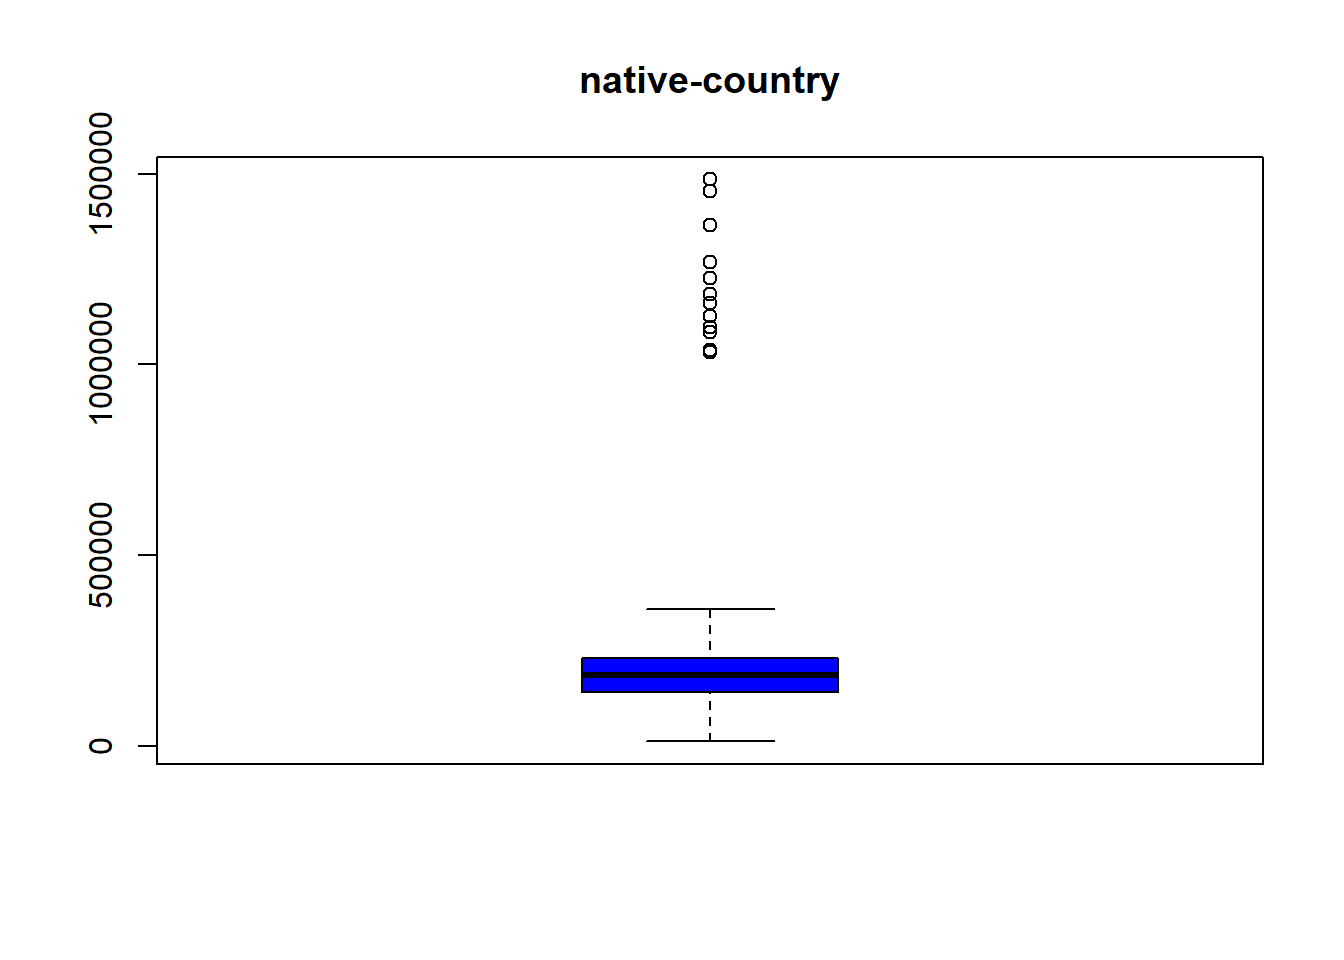
\includegraphics{pra01_Raquel_files/figure-latex/unnamed-chunk-55-1.pdf}
Sigue habiendo algunos datos outliers pero hay que tener en cuenta que
la mayoría de nuestro data frame se concentra en norte américa. Vamos a
ver los porcentajes.

\begin{Shaded}
\begin{Highlighting}[]
\KeywordTok{prop.table}\NormalTok{(}\KeywordTok{table}\NormalTok{(df1}\OperatorTok{$}\StringTok{\textasciigrave{}}\DataTypeTok{native{-}country}\StringTok{\textasciigrave{}}\NormalTok{))}
\end{Highlighting}
\end{Shaded}

\begin{verbatim}
## 
##        Asia      Europa Nor_America       Otros Sur_America 
##  0.02063559  0.01617800  0.89843600  0.02248011  0.04227030
\end{verbatim}

El 89,84\% de los datos pertenecen a norte América, por lo que es lógico
que existan outliers que, en este caso, no vamos a eliminar.

\hypertarget{income}{%
\subsubsection{income}\label{income}}

La variable ingresos Income, solo diferencia entre menor o igual de 50k,
no sabemos cuál es la moneda de referencia, y más de 50k. Vemos que el
porcentaje de menor o igual de 50k es superior al de observaciones que
cobran más de esa cantidad:

\begin{Shaded}
\begin{Highlighting}[]
\KeywordTok{round}\NormalTok{(}\KeywordTok{prop.table}\NormalTok{(}\KeywordTok{table}\NormalTok{(df1}\OperatorTok{$}\NormalTok{income))}\OperatorTok{*}\DecValTok{100}\NormalTok{, }\DecValTok{2}\NormalTok{)}
\end{Highlighting}
\end{Shaded}

\begin{verbatim}
## 
##  <=50K   >50K 
##  75.56  24.44
\end{verbatim}

Exactamente un 75.92\% de las observaciones cobran menos o igual de 50k
y un 24.08\% cobra más.

Vamos a ver por continentes, cuáles tienes mayores ingresos.

\begin{Shaded}
\begin{Highlighting}[]
\KeywordTok{table}\NormalTok{(df1}\OperatorTok{$}\StringTok{\textasciigrave{}}\DataTypeTok{native{-}country}\StringTok{\textasciigrave{}}\NormalTok{, df1}\OperatorTok{$}\NormalTok{income)}
\end{Highlighting}
\end{Shaded}

\begin{verbatim}
##              
##                <=50K  >50K
##   Asia           365   172
##   Europa         303   118
##   Nor_America  17532  5848
##   Otros          447   138
##   Sur_America   1015    85
\end{verbatim}

Y en porcentajes

\begin{Shaded}
\begin{Highlighting}[]
\NormalTok{A \textless{}{-}}\StringTok{ }\KeywordTok{round}\NormalTok{(}\KeywordTok{prop.table}\NormalTok{(}\KeywordTok{table}\NormalTok{(df1}\OperatorTok{$}\StringTok{\textasciigrave{}}\DataTypeTok{native{-}country}\StringTok{\textasciigrave{}}\NormalTok{, df1}\OperatorTok{$}\NormalTok{income))}\OperatorTok{*}\DecValTok{100}\NormalTok{,}\DecValTok{2}\NormalTok{)}
\NormalTok{A}
\end{Highlighting}
\end{Shaded}

\begin{verbatim}
##              
##                <=50K  >50K
##   Asia          1.40  0.66
##   Europa        1.16  0.45
##   Nor_America  67.37 22.47
##   Otros         1.72  0.53
##   Sur_America   3.90  0.33
\end{verbatim}

Vamos a verlo gráficamente.

\begin{Shaded}
\begin{Highlighting}[]
\KeywordTok{ggplot}\NormalTok{(}\DataTypeTok{data=}\NormalTok{df1[}\DecValTok{1}\OperatorTok{:}\NormalTok{filas,],}\KeywordTok{aes}\NormalTok{(}\DataTypeTok{x=}\StringTok{\textasciigrave{}}\DataTypeTok{native{-}country}\StringTok{\textasciigrave{}}\NormalTok{, }\DataTypeTok{fill=}\NormalTok{ income ))}\OperatorTok{+}\KeywordTok{geom\_bar}\NormalTok{()}
\end{Highlighting}
\end{Shaded}

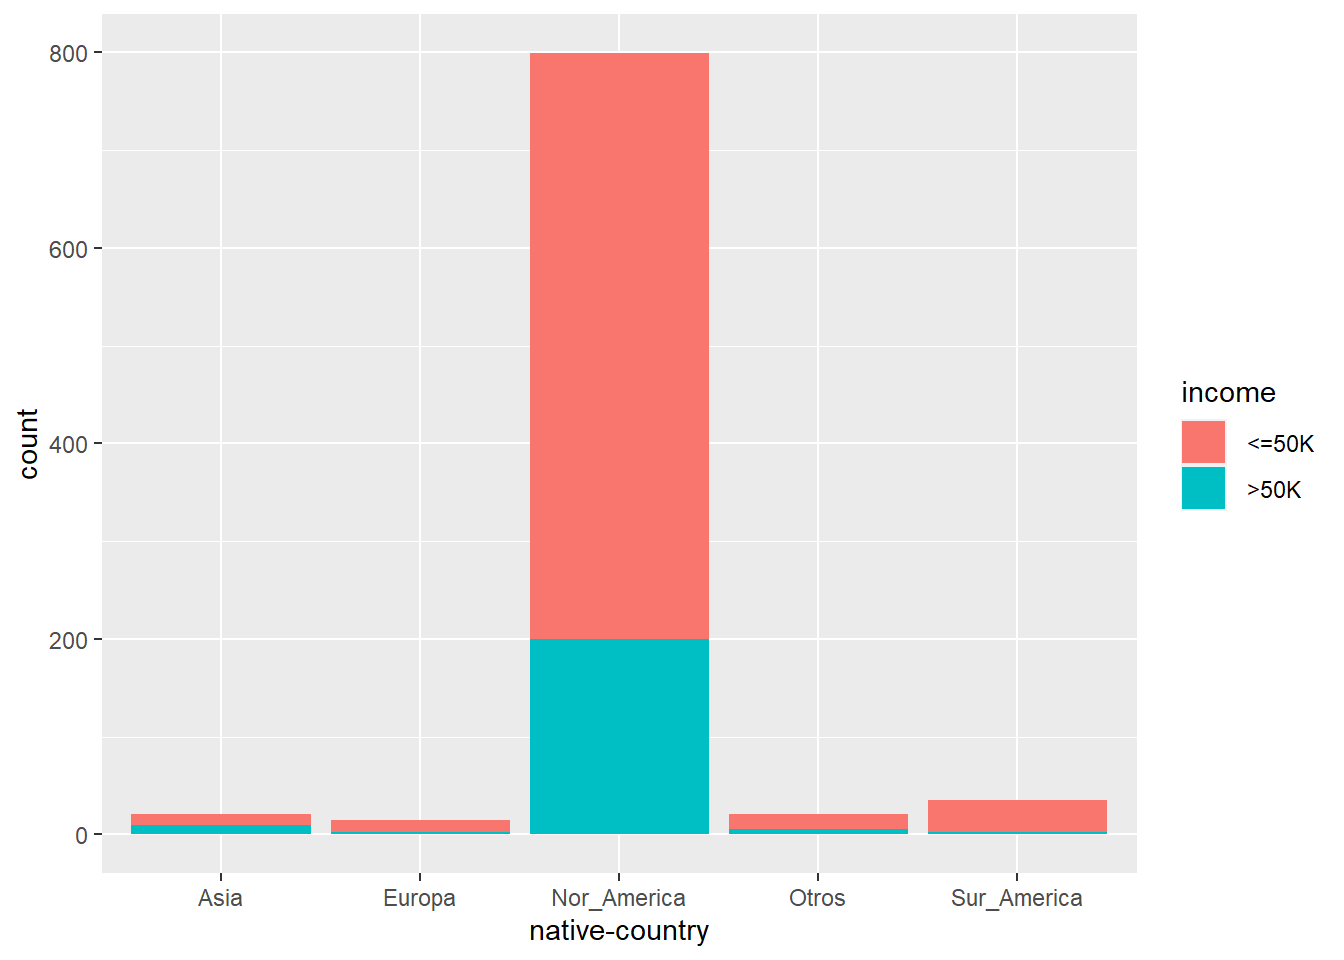
\includegraphics{pra01_Raquel_files/figure-latex/unnamed-chunk-60-1.pdf}

Vemos que como la mayoría de datos están recogidos en norte América, es
complicado ver el resto de datos.


\end{document}
